\documentclass[11pt]{article}
\usepackage{amsmath,amssymb,amsthm,booktabs,geometry,graphicx}
\usepackage[utf8]{inputenc}
\usepackage[T1]{fontenc}
\usepackage[french]{babel}
\usepackage[round,authoryear]{natbib}
\usepackage[colorlinks=true,linkcolor=black,citecolor=black,urlcolor=blue!50!black]{hyperref}
\geometry{margin=1in}

\newtheorem{proposition}{Proposition}
\newtheorem{assumption}{Hypothèse}
\theoremstyle{definition}
\newtheorem{postulate}{Postulat}
\newtheorem{definition}{Définition}
\renewcommand{\proofname}{Démonstration}

\newcommand{\JJ}{\mathcal{J}}
\newcommand{\DD}{\mathcal{D}}
\newcommand{\Dun}{\mathcal{D}_1}
\newcommand{\KL}[2]{D_{KL}\!\left(#1\,\Vert\,#2\right)}

\title{Sauts d'entropie et relaxation de l'information sur les marchés financiers :\\
du maximum d'entropie en temps-volume aux tests de résistance calibrés en entropie}
\author{Version de travail}
\date{Août 2026}

\begin{document}
\maketitle

\begin{abstract}
\noindent Cet article reconstruit la lecture informationnelle de la formation
des prix autour d'une seule asymétrie. Nous fermons d'abord le pont qui mène du
maximum d'entropie aux prix gaussiens, là où il est habituellement laissé
ouvert, en définissant le prix comme un flux d'ordres accumulé et en appliquant
le principe de maximum d'entropie en \emph{temps-volume} plutôt qu'en temps
calendaire : le volume échangé fixant le budget de variance, la distribution
conditionnelle la moins engageante de l'incrément de log-prix est gaussienne, et
la cohérence temporelle fait alors du log-prix un mouvement brownien subordonné
à l'horloge de volume, donc du prix un mouvement brownien géométrique. Lu à
l'envers, le même argument dit que des prix non gaussiens sont la signature
d'une distribution conditionnelle qui n'est \emph{pas} d'entropie maximale,
c'est-à-dire d'une information contraignante.

Nous décomposons ensuite l'entropie d'un vecteur de rendements en trois canaux :
l'échelle ($\sum_i\log\sigma_i$), la dépendance ($\tfrac12\log\det R \le 0$) et
la forme (le déficit d'entropie $\DD=\KL{p}{q}$, qui n'est autre que
l'asymétrie et les queues épaisses). La combinaison des deux derniers donne un
indice structurel sans échelle
$\JJ_t = \DD_t - \tfrac12\log\det R_t = \KL{p_t}{\prod_i q_{i,t}} \ge 0$,
qui mesure la distance du marché à la référence d'entropie maximale à
volatilité inchangée. Puisque conditionner ne peut pas augmenter l'entropie
espérée, un événement informationnel abaisse l'entropie conditionnelle
\emph{moyenne} d'exactement l'information mutuelle de la nouvelle, et abaisse au
sens large le plafond de maximum d'entropie à chaque réalisation : les sauts
d'entropie vers le bas sont un théorème, non une hypothèse. Ce que nous postulons, c'est l'autre moitié : que
l'entropie remonte par diffusion (P1), et que la contrainte imposée par la
nouvelle est unilatérale, de sorte qu'un saut s'accompagne d'une asymétrie
négative (P2). Ensemble, ces éléments donnent à $\JJ$ une dynamique de saut et
diffusion de type Barndorff-Nielsen--Shephard : hausses par sauts, baisses par
diffusion.

Sept hypothèses sont testées sur 33 ans de rendements quotidiens d'actions
individuelles (vingt composantes du S\&P~500, 1990--2022), répliquées sur le
panel \texttt{EuStockMarkets} et --- c'est là l'essentiel --- jugées face à deux
témoins calibrés construits en rééchantillonnant les rendements observés : l'un
i.i.d., qui conserve les queues marginales épaisses et détruit toute structure
temporelle, l'autre par blocs de 21~jours, qui conserve en outre le
regroupement de volatilité. Pris au pied de la lettre, les résultats paraissent
solides : le stress élève $\JJ$ de 2,89~nats, les variations de $\JJ$ sont
massivement unilatérales (158 sauts positifs contre 9 négatifs, asymétrie
$+12{,}3$), les sauts positifs s'accompagnent d'une asymétrie de marché
négative, et les canaux de dépendance et de queue se verrouillent sous stress
($0{,}04$ en marché calme contre $0{,}66$). Face aux témoins, l'essentiel
s'évapore. L'asymétrie des sauts, la signature d'asymétrie et le couplage des
canaux sont tous reproduits --- plusieurs sont même \emph{dépassés} --- par des
données rééchantillonnées, parce qu'une fonctionnelle convexe positive de
moments estimés monte brutalement et redescend en douceur dès qu'une observation
à queue épaisse entre dans l'estimateur. Exactement deux statistiques franchissent
les deux témoins, et ce sont celles qu'il faut retenir : l'écart de régime du
canal de \emph{dépendance} ($-1{,}72$~nats contre $-0{,}29$ et $-0{,}64$) et
l'étendue de $\JJ$ sur l'échantillon ($18{,}95$ contre $10{,}49$ et $14{,}23$).
Ce qui distingue une crise d'une simple série de gros rendements, c'est que la
coupe transversale se couple --- le nombre effectif de modes de risque
indépendants tombe de $13{,}2$ à $10{,}5$ sur $20$ --- et non que les
marginales s'épaississent. La demi-vie de relaxation n'est pas identifiée : à
$120$~jours, elle se situe au-dessus du témoin i.i.d.\ ($92$) et en dessous du
témoin par blocs ($162$). Deux autres résultats vont à l'encontre de l'intérêt de
l'article : la compensation volatilité--dépendance observée sur des portefeuilles
sectoriels ne se réplique pas sur des titres individuels, et aucun canal
d'entropie n'améliore hors échantillon la prévision du risque futur par rapport à
une référence de volatilité.

La contribution appliquée est une construction de test de résistance. Un scénario
de sévérité $\eta$ est la pire distribution conditionnelle contenue dans une
boule de Kullback--Leibler de rayon $\eta$~nats autour de la distribution
conditionnelle courante du marché ; le rayon est calibré sur le flux
d'information réalisé du marché lui-même, $\KL{p_t}{p_{t-h}}$, de sorte qu'une
sévérité porte une période de retour plutôt qu'un adjectif, et que le
déplacement de la moyenne et l'inflation de la variance sont prélevés sur un
même budget au lieu d'être choqués séparément. Un nat achète $\sqrt2$~sigma. La
même métrique tarife les scénarios existants : un bundle classique --- volatilités
doublées, toutes les corrélations forcées à $0{,}9$, un choc de trois sigmas ---
se tarife à $9{,}97$~nats, entre les échelons vicennal et cinquantennal, mais
délivre une perte de queue qu'un scénario entropique atteint pour $5{,}47$ ; le
comité a acheté une perte décennale au prix d'une invraisemblance trentennale.
Nous décomposons ce prix pour montrer où il passe, et la composante chère n'est
pas celle que l'intuition désigne.
\end{abstract}

\tableofcontents

\section*{Notations}
\addcontentsline{toc}{section}{Notations}

\noindent Deux mises en garde avant le tableau. D'abord, l'entropie
différentielle $h$ \textbf{dépend des unités} : $h(aX)=h(X)+\log|a|$, de sorte
qu'exprimer les rendements en pourcentages plutôt qu'en décimales déplace $h$
d'une constante. Les divergences ($\KL{\cdot}{\cdot}$, $I$, $\DD$, $\JJ$) sont au
contraire invariantes par tout changement de variable inversible : c'est la
raison d'être de l'indice structurel. Ensuite, $K$ désigne un kurtosis et les
lettres \og KL \fg{} sont les initiales de Kullback et Leibler ; il n'y a aucun
lien entre les deux.

\begin{center}
\small
\begin{tabular}{@{}lll@{}}
\toprule
Symbole & Signification & Nature \\
\midrule
$p_t$ & loi conditionnelle vraie des rendements en $t$ & --- \\
$q_t$ & gaussienne de mêmes moyenne et covariance que $p_t$ & --- \\
$h(\cdot)$ & entropie différentielle & nats, \emph{dépend des unités} \\
$\KL{p}{q}$ & divergence de Kullback--Leibler & nats, invariante \\
$\DD_t$ & déficit d'entropie $=\KL{p_t}{q_t}\ge0$ & nats, invariante \\
$\Dun(z)$ & déficit d'un scalaire standardisé (néguentropie) & nats, invariante \\
$H^{vol}_t$ & canal d'échelle $=\sum_i\log\sigma_{i,t}$ & nats, \emph{dépend des unités} \\
$H^{dep}_t$ & canal de dépendance $=\tfrac12\log\det R_t\le0$ & nats, invariante \\
$H^{cov}_t$ & $H^{vol}_t+H^{dep}_t$ ; la constante $\tfrac N2\log2\pi e$ est omise & nats \\
$\JJ_t$ & indice structurel $=\DD_t-H^{dep}_t\ge0$ & nats, invariante \\
$I(X;Y)$ & information mutuelle & nats, invariante \\
$I^{(h)}_t$ & flux d'information $=\KL{p_t}{p_{t-h}}$ & nats \\
$S$, $K$ & asymétrie, kurtosis excédentaire & sans dimension \\
$\Sigma_t=D_tR_tD_t$ & covariance, écarts types, corrélation & --- \\
$\lambda_k$, $N^{\text{eff}}_t$ & valeurs propres de $R_t$, nombre effectif de modes & $1\le N^{\text{eff}}\le N$ \\
$\kappa$, $\sigma_\JJ$ & taux de relaxation et coefficient de diffusion de $\JJ$ & --- \\
$\eta$ & rayon d'un scénario de stress & nats \\
$N$ & nombre d'actifs & --- \\
\bottomrule
\end{tabular}
\end{center}

\section{Introduction}
\label{sec:intro}

Deux faits relatifs aux prix financiers cohabitent mal. Le premier est que le
modèle gaussien est la réponse naturelle à une question d'ignorance : fixez une
moyenne et une variance, ne sachez rien d'autre, et la distribution de maximum
d'entropie est gaussienne. Le second est que les rendements ne sont pas
gaussiens : ils ont des queues épaisses, une asymétrie négative, et leur
dépendance se resserre précisément quand cela compte.

La réaction habituelle consiste à traiter le second fait comme un défaut du
premier modèle et à le rapiécer : ajouter des sauts au prix, ajouter un facteur
de volatilité stochastique, ajouter une copule. Cet article prend le chemin
inverse. Si le gaussien est ce que délivre le maximum d'entropie, alors tout
écart au gaussien est une mesure de la distance du marché à l'ignorance
maximale, c'est-à-dire une mesure d'information. La question n'est donc pas
comment rapiécer le gaussien, mais comment lire la taille, la dynamique et la
direction de l'écart.

L'article s'organise autour d'une asymétrie de cet écart. L'information arrive
par paquets et s'absorbe graduellement. Une surprise de banque centrale, un
défaut, une guerre supprime l'incertitude en un instant ; le marché passe ensuite
des semaines à en déduire les implications, et l'incertitude se reconstitue. Si
l'entropie est la bonne monnaie de l'incertitude, sa dynamique devrait être en
dents de scie : chutes brutales, remontées lentes. Cette forme n'est pas un fait
stylisé qu'il aurait fallu supposer --- la moitié en est un théorème. Conditionner
ne peut pas augmenter l'entropie espérée, donc l'arrivée d'un signal abaisse
l'entropie conditionnelle \emph{moyenne} d'exactement l'information mutuelle
entre le signal et le prix (proposition~\ref{prop:conditioning}) ; et le plafond
de maximum d'entropie, lui, baisse au sens large à chaque réalisation, sans
qu'on puisse en général quantifier cette baisse (proposition~\ref{prop:constraint}).
Les deux énoncés sont distincts et l'annexe~\ref{app:mi} les sépare
explicitement, avec un exemple gaussien chiffré. La taille \emph{espérée} du
saut, en nats, est le contenu informationnel de la nouvelle. Ce qu'il faut
postuler, c'est la remontée et la direction.

Trois contributions en découlent.

\paragraph{Le pont volume (section~\ref{sec:bridge}).}
Le passage de \og le maximum d'entropie donne un gaussien \fg{} à \og les prix
sont gaussiens \fg{} est couramment affirmé et rarement argumenté, parce que le
maximum d'entropie est un énoncé sur une distribution à variance fixée et ne dit
rien de l'origine de cette variance. Nous le fermons en définissant le prix comme
un flux d'ordres accumulé et en appliquant le principe en temps-volume : le
volume total échangé, qui est observable, fixe le budget de variance, et
l'incrément de maximum d'entropie conditionnel au volume est gaussien de variance
proportionnelle au volume. C'est l'hypothèse de mélange de distributions
\citep{clark1973,tauchen1983,ane2000}, déduite plutôt que supposée. La cohérence
temporelle fait ensuite du log-prix un mouvement brownien subordonné à l'horloge
de volume, et le lemme d'Itô fait du prix un mouvement brownien géométrique. Le
pont explique aussi, dans la même phrase, pourquoi les rendements en temps
calendaire ne sont pas gaussiens : soit la distribution conditionnelle n'est pas
d'entropie maximale (l'information contraint), soit l'horloge de volume est
aléatoire, soit les deux --- et les deux sources laissent des empreintes
différentes.

\paragraph{Trois canaux et un indice sans échelle (section~\ref{sec:channels}).}
L'entropie gaussienne d'un vecteur de rendements se scinde exactement en un
terme d'échelle et un terme de dépendance, et l'entropie véritable en diffère du
déficit d'entropie $\DD=\KL{p}{q}$, où logent l'asymétrie et les queues épaisses.
Le terme d'échelle domine le niveau de l'entropie différentielle et n'apprend
rien sur l'information ; en le retirant, il reste
$\JJ = \DD - \tfrac12\log\det R$, qui est exactement $\KL{p}{\prod_i q_i}$ ---
la divergence à un produit de marginales gaussiennes de mêmes échelles. $\JJ$ est
positif, invariant au niveau de volatilité, et additif sur ses deux canaux
destructeurs d'entropie. C'est la variable d'état dont traite le reste de
l'article. Empiriquement, il ne partage que $21\%$ de sa variance avec la
volatilité, et son canal de forme est essentiellement orthogonal à la volatilité
($r=0{,}09$).

\paragraph{Tests de résistance en nats (section~\ref{sec:stress}).}
Un scénario de sévérité $\eta$ est la pire distribution conditionnelle contenue
dans une boule KL de rayon $\eta$ autour de celle d'aujourd'hui. La construction
n'est pas nouvelle \citep{glasserman2014,breuer2013} ; la calibration l'est. Le
rayon se lit sur le flux d'information réalisé du marché, la révision à $h$ pas
$\KL{p_t}{p_{t-h}}$, mesurée dans la même unité que le rayon, si bien qu'une
sévérité acquiert une période de retour. Parce que le déplacement de moyenne et
l'inflation de variance sont choisis sur un même budget, le scénario ne peut pas
être incohérent en interne, et parce que \emph{tout} scénario peut être tarifé
sur la même échelle, la question \og ce test de résistance est-il assez
sévère ? \fg{} devient arithmétique.

\paragraph{Un avertissement sur la mesure de tout ceci.}
L'indice structurel est une fonctionnelle convexe positive de moments d'ordre
deux, trois et quatre estimés. Le bruit d'estimation sur des données à queues
épaisses pousse une telle fonctionnelle \emph{vers le haut} brutalement et la
laisse décroître \emph{en douceur}, ce qui est précisément la dent de scie que
prédisent les postulats. Chaque statistique de saut et de relaxation ci-dessous
est donc rapportée face à un témoin construit en rééchantillonnant les rendements
observés --- en conservant les queues marginales, en détruisant la chronologie. Le
résultat est inconfortable et, nous le pensons, la chose la plus utile de
l'article : l'asymétrie des sauts, qui paraît écrasante, ne survit pas ; la
persistance et l'amplitude, si. Quiconque construit un indicateur de crise à
partir d'une fonctionnelle convexe de moments estimés devrait faire tourner ce
témoin avant de croire son propre graphique.

La section~\ref{sec:dynamics} énonce le théorème et les deux postulats et en
dérive la dynamique de saut-diffusion ; la section~\ref{sec:hypotheses} liste les
hypothèses ; les sections~\ref{sec:data}--\ref{sec:results} donnent les données,
les estimateurs et les résultats, dont le témoin placebo que les statistiques de
saut et de relaxation doivent franchir ; la section~\ref{sec:stress} construit le
test de résistance ; la section~\ref{sec:limits} est honnête sur ce que rien de
tout ceci n'établit.

\section{Du flux d'ordres au prix gaussien : le pont volume}
\label{sec:bridge}

\subsection{Le prix comme flux d'ordres accumulé}

Sur $[t,t+\Delta]$, soit $M$ le nombre de transactions exécutées, la transaction
$k$ portant le volume signé $\epsilon_k v_k$ avec $\epsilon_k\in\{-1,+1\}$ le
sens (à l'initiative de l'acheteur ou du vendeur) et $v_k>0$ la taille. Notons
$V=\sum_k v_k$ le volume total et $Q=\sum_k \epsilon_k v_k$ le flux d'ordres
signé net.

\begin{assumption}[Impact linéaire]\label{as:impact}
Le log-prix répond linéairement au flux d'ordres signé net,
$\Delta X_{t,\Delta} = X_{t+\Delta}-X_t = \lambda\,Q$, avec $\lambda>0$ constant
sur l'intervalle.
\end{assumption}

C'est l'équilibre de \citet{kyle1985} : le teneur de marché, incapable de
distinguer le flux informé du flux non informé, fixe une règle de prix linéaire
et $\lambda$ est l'inverse de la profondeur. C'est la définition du \og prix
comme fonction du volume échangé \fg{} dont a besoin le reste de la section, et
c'est le maillon le plus faible de la chaîne ; la
section~\ref{sec:bridge-caveats} dit ce qui se passe quand il cède.

\begin{assumption}[Signes échangeables et variance proportionnelle au volume]
\label{as:signs}
Conditionnellement à $V$ et à l'information disponible en $t$, la croyance du
marché sur $Q$ n'est contrainte que par ses deux premiers moments, avec
$\mathbb{E}[Q\mid V] = m$ et $\mathrm{Var}(Q\mid V) = \varsigma^2 V$.
\end{assumption}

La forme de la variance est celle qu'on obtient lorsque les signes des
transactions sont échangeables à corrélation bornée et que les tailles ont une
moyenne stable : pour des signes indépendants,
$\mathrm{Var}(Q)=\sum_k v_k^2 \approx \bar v V$. Le contenu économique est que
\emph{le volume, et non le temps, est la mesure naturelle de ce qui peut se
produire}.

\subsection{Maximum d'entropie en temps-volume}

\begin{proposition}[Maximum d'entropie sous contraintes de moments d'ordre un et deux]
\label{prop:maxent}
Parmi les distributions absolument continues sur $\mathbb{R}^N$ de moyenne $\mu$
et de covariance $\Sigma\succ0$, la gaussienne $\mathcal N(\mu,\Sigma)$ maximise
de façon unique l'entropie différentielle, et
$h^{\max}(\Sigma)=\tfrac12\log\left((2\pi e)^N\det\Sigma\right)$.
\end{proposition}

\begin{proof}
Soit $q=\mathcal N(\mu,\Sigma)$ et soit $p$ de mêmes deux premiers moments et
d'entropie différentielle finie. Comme $\log q$ est exactement quadratique, son
espérance ne dépend que de ces moments, donc
$\mathbb{E}_p[\log q]=\mathbb{E}_q[\log q]=-h(q)$. La positivité de l'entropie
relative donne $0\le \KL{p}{q} = -h(p)+h(q)$, d'où $h(p)\le h(q)$, avec égalité
si et seulement si $p=q$ presque partout. L'argument n'exige aucune
différentiabilité de $p$ ni l'existence préalable d'un maximiseur.
\end{proof}

La voie variationnelle --- un lagrangien sur les contraintes de normalisation, de
moyenne et de covariance, dont la condition du premier ordre rend $\log p$
quadratique --- explique \emph{pourquoi} le maximiseur est gaussien, mais c'est
l'argument par la divergence qui établit l'optimalité et l'unicité.

En appliquant la proposition~\ref{prop:maxent} à
l'hypothèse~\ref{as:signs} en dimension un, puis en transportant par
l'hypothèse~\ref{as:impact} :

\begin{equation}
\label{eq:mdh}
\Delta X_{t,\Delta}\ \big|\ V \ \sim\ \mathcal{N}\!\left(\lambda m,\ \lambda^2\varsigma^2 V\right).
\end{equation}

L'équation~\eqref{eq:mdh} est le pont. Trois points méritent d'être soulignés.

D'abord, \emph{la variable de conditionnement est le volume, pas le temps}. Le
maximum d'entropie ne délivre pas une variance ; il délivre la distribution la
moins engageante étant donné une variance. L'hypothèse~\ref{as:signs} fournit
cette variance à partir d'un observable, et cet observable est le volume échangé.
L'équation~\eqref{eq:mdh} est l'hypothèse de mélange de distributions de
\citet{clark1973} et \citet{tauchen1983}, obtenue ici comme un énoncé de maximum
d'entropie plutôt que posée ; \citet{ane2000} montrent empiriquement que les
rendements mesurés en temps-transaction sont proches du gaussien alors que les
rendements en temps calendaire ne le sont pas, ce qui est la prédiction
de~\eqref{eq:mdh}.

Ensuite, \emph{la gaussianité est conditionnelle}. Inconditionnellement,
$\Delta X$ est un mélange d'échelle de lois normales sur le volume aléatoire $V$,
donc leptokurtique même si \eqref{eq:mdh} est exacte. C'est le mécanisme de
subordination de \citet{mandelbrot1967}, et cela signifie que les queues épaisses
ne constituent pas à elles seules une preuve contre le maximum d'entropie.

Enfin, l'extension multivariée est immédiate : avec $N$ actifs,
$\Delta \mathbf{X}\mid V \sim \mathcal N(\boldsymbol\mu V, \Sigma V)$, et la
proposition~\ref{prop:maxent} s'applique telle quelle.

\subsection{Des incréments gaussiens au mouvement brownien puis au MBG}

Soit $\theta_t=\int_0^t v_s\,ds$ l'horloge de volume cumulé.
L'équation~\eqref{eq:mdh} donne la loi d'un incrément ; un processus demande
davantage.

\begin{assumption}[Cohérence temporelle]\label{as:time}
Dans l'horloge de volume, les incréments sur des intervalles disjoints sont
indépendants, les trajectoires sont continues, et la covariance d'un incrément
est proportionnelle au volume écoulé.
\end{assumption}

Sous l'hypothèse~\ref{as:time} à coefficients constants, il existe une matrice
$B$ telle que $BB^{\!\top}=\Sigma$ et $X_\theta = X_0 + \mu\theta + BW_\theta$ en
temps-volume, donc en temps calendaire
\begin{equation}
\label{eq:subordination}
X_t = X_0 + \mu\,\theta_t + B\,W_{\theta_t},
\end{equation}
un mouvement brownien \emph{subordonné} à l'horloge de volume. Si l'intensité de
négociation est constante, $\theta_t=\bar v\,t$ et \eqref{eq:subordination} est
un mouvement brownien ordinaire en temps calendaire ; en exponentiant et en
appliquant Itô,
\begin{equation}
\frac{dS_{i,t}}{S_{i,t}} = \left(a_{i,t}+\tfrac12\sigma_{i,t}^2\right)dt + \sigma_{i,t}\,dW_{i,t},
\end{equation}
de sorte que la dérive du prix n'est pas celle du log-prix --- la même correction
du second ordre qui reparaîtra à la section~\ref{sec:channels} lorsqu'on
différenciera $\log\det R_t$.

Il vaut la peine d'être précis sur ce que fait l'hypothèse~\ref{as:time}. Par le
théorème de \citet{monroe1978}, \emph{toute} martingale locale continue est un
mouvement brownien changé de temps : la subordination seule n'a donc aucun
contenu empirique. Le contenu est dans l'horloge : \eqref{eq:mdh} dit que la
bonne horloge est le volume, et l'hypothèse~\ref{as:time} dit que le marché est
sans mémoire dans cette horloge. C'est le maximum d'entropie qui sélectionne le
mouvement brownien dans la classe qu'autorise le théorème de Monroe.

\subsection{La contraposée}
\label{sec:contrapositive}

La proposition~\ref{prop:maxent} se lit dans les deux sens. Notons $q_t$ la
gaussienne de mêmes moyenne et covariance conditionnelles que $p_t$. Alors

\begin{equation}
\label{eq:deficit}
\DD_t \;\equiv\; h(q_t) - h(p_t) \;=\; \KL{p_t}{q_t} \;\ge\; 0,
\end{equation}
avec égalité si et seulement si $p_t$ est gaussienne. Donc : \emph{les prix sont
non gaussiens exactement dans la mesure où leur distribution conditionnelle n'est
pas d'entropie maximale}, et $\DD_t$ mesure cette mesure. Dans le langage de la
section~\ref{sec:bridge}, un $\DD_t$ positif signifie que des contraintes
au-delà des deux premiers moments sont actives --- que quelqu'un sait quelque
chose que le moment d'ordre deux n'encode pas.

Deux sources produisent un déficit positif, et les séparer importe. Une horloge
de volume aléatoire produit un mélange d'échelle, symétrique et leptokurtique.
Une information directionnelle contraignante produit de l'asymétrie. La
section~\ref{sec:channels} scinde $\DD$ exactement selon cette ligne.

\subsection{Où le pont est faible}
\label{sec:bridge-caveats}

L'hypothèse~\ref{as:impact} est linéaire ; l'impact empirique d'un métaordre est
plus proche d'une racine carrée de la taille, ce qui rend concave l'application
du flux au prix et la distribution de rendements induite moins épaisse en queue
que le flux. L'hypothèse~\ref{as:signs} traite les signes comme échangeables ;
le flux d'ordres est en réalité fortement autocorrélé, ce qui gonfle
$\mathrm{Var}(Q)$ au-dessus de $\varsigma^2 V$ et fait de l'horloge de volume un
substitut imparfait de la variance. Aucune de ces défaillances ne change la
\emph{forme} de l'argument --- le maximum d'entropie sous budget de variance
reste gaussien --- mais toutes deux signifient que l'horloge de volume est une
approximation de l'horloge d'information plutôt que cette horloge même. Nous
utilisons le raisonnement en temps-volume pour motiver le cadre et l'estimation
en temps calendaire dans tout le travail empirique, de sorte qu'aucun résultat
ci-dessous ne dépend de l'exactitude de \eqref{eq:mdh}.

\section{Les trois canaux de l'entropie}
\label{sec:channels}

\subsection{Échelle et dépendance}

Écrivons $\Sigma_t = D_tR_tD_t$ avec
$D_t=\mathrm{diag}(\sigma_{1,t},\dots,\sigma_{N,t})$. Alors
$\det\Sigma_t = \left(\prod_i\sigma_{i,t}^2\right)\det R_t$ et
\begin{equation}
\label{eq:ceiling}
h(q_t) \;=\; \underbrace{\tfrac{N}{2}\log(2\pi e)}_{\text{constante}}
\;+\; \underbrace{\sum_i \log\sigma_{i,t}}_{H^{vol}_t}
\;+\; \underbrace{\tfrac12\log\det R_t}_{H^{dep}_t}.
\end{equation}
Par l'inégalité de Hadamard, $H^{dep}_t\le 0$, avec égalité si et seulement si
$R_t=I$ : \emph{la corrélation détruit toujours de l'entropie}, et $-H^{dep}_t$
est précisément la multi-information gaussienne (corrélation totale) du vecteur
de rendements. Une lecture utile de la même quantité est spectrale : avec
$\lambda_k$ les valeurs propres de $R_t$ et $\tilde\lambda_k=\lambda_k/N$, le
nombre de participation
$N^{\text{eff}}_t=\exp\!\left(-\sum_k\tilde\lambda_k\log\tilde\lambda_k\right)$
est le nombre effectif de modes de risque indépendants ; il vaut $N$ pour $R=I$
et tend vers $1$ lorsqu'un unique mode collectif absorbe la variance.

L'équation~\eqref{eq:ceiling} est le plafond, pas l'entropie. C'est ce
qu'implique la seule matrice de covariance, et la proposition~\ref{prop:maxent}
dit que la vérité se situe en dessous.

\subsection{Forme : le déficit d'entropie et sa composition}

En soustrayant \eqref{eq:deficit} de \eqref{eq:ceiling} on obtient la
décomposition de l'article, trois canaux et une constante :
\begin{equation}
\label{eq:three}
h(p_t) \;=\; \tfrac{N}{2}\log(2\pi e) \;+\; \underbrace{H^{vol}_t}_{\text{échelle}} \;+\; \underbrace{H^{dep}_t}_{\text{dépendance}} \;-\; \underbrace{\DD_t}_{\text{forme}}.
\end{equation}

Le canal de forme, ce sont l'asymétrie et les queues épaisses, et le
développement d'Edgeworth le dit explicitement : pour une variable standardisée
d'asymétrie $S$ et de kurtosis excédentaire $K$ au voisinage de la gaussianité,
\begin{equation}
\label{eq:edgeworth}
J \;\approx\; \frac{S^2}{12} + \frac{K^2}{48}.
\end{equation}
L'équation~\eqref{eq:edgeworth} répond à la question \og où un saut d'entropie
serait-il visible ? \fg{} : dans les moments d'ordre trois et quatre, de manière
additive, avec un canal d'asymétrie et un canal de queue. Elle est aussi la
source du problème de signe que la section~\ref{sec:dynamics} doit résoudre, car
$S$ y entre au carré --- \emph{la néguentropie ne distingue pas un krach d'une
envolée}. Comme estimateur, \eqref{eq:edgeworth} est inutilisable sur des
rendements quotidiens ; la section~\ref{sec:estimators} documente à quel point et
ce que nous utilisons à la place.

\subsection{L'indice structurel}

Le canal d'échelle est une nuisance pour notre propos : il domine numériquement
le niveau de \eqref{eq:three}, il bouge avec la volatilité, et un changement
d'unités le modifie. Les deux autres canaux sont sans échelle. En les combinant,
et en utilisant la règle de chaînage exacte
$\KL{p}{\prod_i q_i} = \sum_i \KL{p_i}{q_i} + I(x)$ où $I$ est la
multi-information :

\begin{definition}[Indice d'information structurelle]
\label{def:J}
\begin{equation}
\JJ_t \;\equiv\; \DD_t \;-\; H^{dep}_t \;=\; \KL{p_t}{\textstyle\prod_i q_{i,t}} \;\ge\; 0 ,
\end{equation}
la divergence de la loi jointe conditionnelle des rendements à un produit de
marginales gaussiennes de mêmes échelles.
\end{definition}

$\JJ$ est nul si et seulement si les rendements sont indépendants et gaussiens ;
il s'élève quand les actifs se couplent, quand les marginales s'épaississent ou
quand elles s'asymétrisent. Il est mesuré en nats, il est invariant au niveau de
volatilité, et il est additif sur ses deux canaux, de sorte qu'on peut toujours
demander quelle part d'un mouvement vient de la dépendance et quelle part de la
forme. C'est la variable d'état de la section~\ref{sec:dynamics}.

\section{Dynamique de l'information : un théorème, deux postulats}
\label{sec:dynamics}

\subsection{Les sauts vers le bas sont un théorème}

Deux énoncés distincts sous-tendent la moitié descendante de la dynamique
postulée. Les confondre est une erreur facile, et les versions antérieures de ce
travail la commettaient ; nous les séparons donc explicitement.

Rappelons d'abord la définition de l'\emph{information mutuelle} entre le
vecteur de rendements $X$ et un signal $Y$ :
\begin{equation}
\label{eq:mi}
I(X;Y) \;=\; \KL{p_{XY}}{p_X\otimes p_Y}
\;=\; \iint p(x,y)\,\log\frac{p(x,y)}{p(x)p(y)}\,dx\,dy ,
\end{equation}
c'est-à-dire la divergence de la loi jointe au produit des marginales : de
combien la loi jointe s'écarte de l'indépendance. Elle est positive, symétrique,
nulle si et seulement si $X\perp Y$, et --- contrairement à $h$ --- invariante par
reparamétrisation inversible. Pour un couple gaussien scalaire de corrélation
$\rho$, $I=-\tfrac12\log(1-\rho^2)$.

\begin{proposition}[Chute de l'entropie conditionnelle moyenne]
\label{prop:conditioning}
Soit $X$ le vecteur de rendements et $Y$ un signal. Alors
\begin{equation*}
\mathbb{E}_Y\!\left[h(X\mid Y)\right] \;=\; h(X) - I(X;Y) \;\le\; h(X),
\end{equation*}
avec égalité si et seulement si $X\perp Y$.
\end{proposition}

\begin{proposition}[Monotonie du plafond sous contrainte]
\label{prop:constraint}
Soient $\mathcal{C}\subseteq\mathcal{C}'$ deux ensembles de contraintes et
$\mathcal{Q}(\cdot)$ l'ensemble des lois qui les satisfont. Alors
$\mathcal{Q}(\mathcal{C}')\subseteq\mathcal{Q}(\mathcal{C})$ et donc
\begin{equation*}
\sup_{p\,\in\,\mathcal{Q}(\mathcal{C}')} h(p) \;\le\; \sup_{p\,\in\,\mathcal{Q}(\mathcal{C})} h(p).
\end{equation*}
\end{proposition}

Les deux résultats sont classiques \citep{cover2006} et ne sont pas
équivalents ; la démonstration détaillée et un exemple gaussien chiffré figurent
en annexe~\ref{app:mi}. Leurs portées diffèrent sur deux axes.

La proposition~\ref{prop:conditioning} \emph{quantifie} la baisse --- exactement
$I(X;Y)$ nats --- mais seulement \emph{en moyenne} sur les réalisations du
signal. Pour un $y$ particulier, $h(X\mid Y=y)$ peut excéder $h(X)$ : un signal
suffisamment déroutant laisse le marché plus incertain qu'avant. Il faut donc
s'attendre à une composante de saut principalement, et non exclusivement,
unilatérale --- ce que trouve la section~\ref{sec:results}.

La proposition~\ref{prop:constraint} vaut au contraire \emph{pour chaque
réalisation}, mais porte sur le \emph{plafond} de maximum d'entropie et non sur
l'entropie réelle, et elle ne quantifie rien : elle dit que le plafond ne peut
pas monter, pas de combien il descend.

Ce que les deux disent ensemble, et qui motive tout ce qui suit : la chute est
\emph{discontinue}, car le signal arrive en un point du temps, et sa taille
espérée en nats est le contenu informationnel de la nouvelle --- une amplitude
mesurée sur une échelle qui ne dépend ni de l'actif, ni de la devise, ni des
unités.

\paragraph{Une réserve d'honnêteté.} Aucune de ces deux propositions n'est
utilisée pour calculer quoi que ce soit dans la partie empirique. Nous mesurons
$\JJ$, et non $h(X)-\mathbb{E}_Y[h(X\mid Y)]$ : estimer une entropie
différentielle en dimension~20 sur une fenêtre de 252~jours est hors de portée
(annexe~\ref{app:units}). Le lien entre le théorème et les statistiques
rapportées plus loin est un raisonnement, pas une identité estimée, et le
lecteur doit le tenir pour tel.

\subsection{Deux postulats}

\begin{postulate}[Relaxation]
\label{p:relax}
En l'absence d'information nouvelle, l'indice structurel décroît vers un niveau
de long terme à taux constant :
$d\JJ_t = -\kappa\left(\JJ_t-\bar\JJ\right)dt + \sigma_\JJ\,dW_t$ avec $\kappa>0$.
\end{postulate}

L'économie derrière P\ref{p:relax} est qu'une contrainte s'évente. La nouvelle
est intégrée aux prix, le désaccord se reforme, les positions se dispersent, et
la coupe transversale recouvre la liberté que le choc lui avait retirée. Rien
dans la théorie de l'information ne délivre cela ; c'est l'hypothèse substantielle
de l'article, et $\kappa$ est l'objet à estimer.

\paragraph{Pourquoi un processus d'Ornstein--Uhlenbeck et pas autre chose ?}
Le choix n'est pas un choix de commodité : il est \emph{forcé} dès qu'on impose
trois exigences minimales, et il est le seul à les satisfaire toutes les trois.

\begin{enumerate}
\item \emph{Markov.} L'avenir de $\JJ$ ne dépend du passé qu'à travers son
niveau présent. C'est l'exigence de parcimonie : ne postuler aucune mémoire
au-delà de ce que l'état courant contient déjà.
\item \emph{Stationnaire.} $\JJ$ possède un niveau de long terme et une variance
finis. Sans cela l'indice dérive, il n'est pas une variable d'état, et les
comparaisons de régime de la section~\ref{sec:results} n'ont pas de sens.
\item \emph{Bruit gaussien.} Entre deux arrivées d'information, on ne prétend
rien savoir du bruit au-delà de sa variance --- c'est le principe de maximum
d'entropie appliqué au bruit lui-même, exactement comme il l'a été aux
rendements en section~\ref{sec:bridge}.
\end{enumerate}

Le théorème de \citet{doob1942} énonce que \textbf{le processus d'Ornstein--Uhlenbeck
est l'unique processus à la fois markovien, gaussien et stationnaire} en temps
continu. Les trois exigences ne laissent donc aucune latitude sur la partie
diffusive : elle est déterminée. Le terme de saut, lui, est ajouté précisément
pour \emph{briser} la gaussianité là où le cadre affirme qu'elle ne tient pas,
c'est-à-dire aux arrivées d'information. La structure de \eqref{eq:ou} est ainsi
un squelette imposé plus une composante délibérément non gaussienne, ce qui est
exactement la classe introduite par \citet{bns2001}.

\paragraph{Ce qui, en revanche, reste arbitraire.} Trois choses, qu'il faut
énoncer plutôt que laisser croire qu'elles découlent du théorème. Le taux
$\kappa$ est supposé \emph{constant} : rien n'interdit qu'une crise soit
absorbée plus vite, ou plus lentement, qu'une nouvelle ordinaire, et les données
employées ici ne permettent pas de trancher. Le rappel est \emph{linéaire} en
l'écart au niveau de long terme, alors qu'un rappel accéléré loin de la moyenne
serait tout aussi plausible. Enfin, $\JJ$ est positif par construction alors
qu'un Ornstein--Uhlenbeck muni d'un terme brownien peut devenir négatif : la
spécification de \citet{bns2001} évite cet écueil en supprimant le terme
brownien et en pilotant le processus par un subordinateur à sauts positifs, ce
qui garantit une loi stationnaire portée par $\mathbb{R}^+$. Empiriquement la
question ne se pose pas --- $\JJ$ reste compris entre $2{,}17$ et $21{,}13$~nats
sur le panel principal et entre $0{,}42$ et $1{,}69$ sur le panel de
réplication, donc très loin de la frontière --- mais formellement il faudrait
soit supprimer $\sigma_\JJ$, soit écrire le processus sur $\log\JJ$.

Le postulat n'est enfin pas anodin sur le plan de la mesure : un estimateur doté
de mémoire fabriquera une décroissance même en l'absence de toute relaxation
économique, aussi la section~\ref{sec:placebo} mesure-t-elle la décroissance
qu'un monde sans mémoire produirait déjà.

\begin{postulate}[Asymétrie de la contrainte]
\label{p:sign}
La contrainte qu'impose l'information est unilatérale dans la direction des
pertes, de sorte qu'un saut d'entropie s'accompagne d'une asymétrie négative du
facteur de marché.
\end{postulate}

\paragraph{Pourquoi ce postulat est logiquement nécessaire.} L'indice $\JJ$ est
une fonction \emph{paire} de l'asymétrie : changer le signe de l'asymétrie ne
change pas sa valeur. La raison est immédiate. Le canal de forme est
$\Dun(z)=\KL{p_z}{\varphi}$, et la loi normale $\varphi$ est symétrique ; donc
si l'on remplace $z$ par $-z$, la loi de référence est inchangée et la
divergence l'est aussi :
\begin{equation}
\label{eq:even}
\Dun(-z)=\Dun(z),\qquad\text{et par conséquent}\qquad \JJ(-x)=\JJ(x).
\end{equation}
Le développement d'Edgeworth \eqref{eq:edgeworth} le rend visible à l'\oe il :
l'asymétrie $S$ y entre au carré.

La conséquence est structurelle et non anecdotique. \textbf{Une distribution à
longue queue à gauche --- un krach --- et son image en miroir à longue queue à
droite --- une envolée --- ont exactement le même $\JJ$.} L'indice mesure la
\emph{taille} de l'information, jamais son sens. Aucun raffinement de
l'estimateur n'y changera quoi que ce soit : c'est une propriété de l'objet
mesuré. Si l'article veut dire quoi que ce soit sur la direction, il doit donc
ajouter un ingrédient extérieur. P\ref{p:sign} est cet ingrédient, et c'est le
plus petit possible : une seule affirmation, sur le signe, ajoutée à un cadre
qui par construction n'en produit aucune.

\paragraph{Sur quoi il s'appuie.} Non pas sur un mécanisme que nous
affirmerions, mais sur une régularité empirique établie : l'\emph{effet de
levier} au sens de \citet{black1976}, c'est-à-dire le fait que les rendements
négatifs sont suivis de hausses de volatilité plus fortes que les rendements
positifs de même amplitude. C'est l'un des faits stylisés les plus robustes de
la finance empirique \citep{christie1982,engle1993,nelson1991}. Traduit dans le
langage de cet article : à quantité d'information égale, la réponse du marché
est plus ample vers le bas que vers le haut, donc un saut de $\JJ$ arrive
accompagné d'une asymétrie de marché négative.

Nous nous abstenons délibérément de choisir entre les explications causales
concurrentes de cet effet --- levier financier à proprement parler, rétroaction
de la volatilité, ou retrait asymétrique de la liquidité du côté vendeur. Le
postulat ne dépend d'aucune d'entre elles : il n'affirme que l'asymétrie, pas sa
cause. Il est testable séparément (H5) et réfutable séparément, et la
section~\ref{sec:results} conclut d'ailleurs qu'il n'est pas établi.

\subsection{La dynamique qui en résulte}

La proposition~\ref{prop:conditioning} jointe à P\ref{p:relax} donne un processus
d'Ornstein--Uhlenbeck non gaussien à sauts unilatéraux, de la classe introduite
par \citet{bns2001} pour la volatilité stochastique :
\begin{equation}
\label{eq:ou}
d\JJ_t \;=\; -\kappa\left(\JJ_t-\bar\JJ\right)dt \;+\; \sigma_\JJ\,dW_t \;+\; \int_{z>0} z\,\mathcal{P}(dt,dz),
\end{equation}
Le terme intégral demande d'être lu avec soin, car sa notation est compacte.

\paragraph{Ce que $\mathcal{P}$ n'est pas.} Ce n'est ni une loi gaussienne, ni
une fonction. La lettre $\mathcal N$ est réservée dans cet article à la loi
normale, et la mesure de saut porte donc un symbole distinct.

\paragraph{Ce que $\mathcal{P}$ est.} Une \emph{mesure aléatoire de comptage},
dite mesure aléatoire de Poisson. On peut se la représenter comme un semis
aléatoire de points dans le plan $(\text{date},\ \text{taille})$ : chaque point
est un événement informationnel, son abscisse est la date à laquelle il survient
et son ordonnée la taille du saut qu'il provoque. Formellement,
$\mathcal{P}(dt,dz)$ vaut $1$ s'il existe un saut dans l'intervalle de temps
$[t,t+dt)$ dont la taille tombe dans $[z,z+dz)$, et $0$ sinon. L'intégrale
$\int_{z>0} z\,\mathcal{P}(dt,dz)$ se lit alors simplement : \og s'il y a un
saut à la date $t$, ajouter sa taille $z$ à $\JJ$ ; sinon n'ajouter rien \fg{}.
C'est une écriture condensée de $\sum_{j} z_j$, la somme des sauts survenus.

\paragraph{Ce qui la caractérise.} Deux ingrédients, réunis dans sa
\emph{mesure d'intensité} $\nu(dz)\,dt$, qui est le nombre espéré de sauts de
taille comprise entre $z$ et $z+dz$ pendant $dt$ : d'une part une
\emph{fréquence d'arrivée} $\lambda=\nu(\mathbb{R}^+)$, en nombre de sauts par
unité de temps, d'autre part une \emph{loi des tailles} $\nu(dz)/\lambda$. Sur
le panel principal, la section~\ref{sec:results} estime $\lambda\approx5$ sauts
par an, une taille moyenne de $0{,}62$~nat et un maximum de $3{,}21$~nats.

\paragraph{Ce qu'est $z$.} La taille d'un saut individuel, exprimée en nats.
Conceptuellement, c'est l'information mutuelle de la nouvelle qui l'a provoqué,
au sens de la proposition~\ref{prop:conditioning}. Opérationnellement, c'est la
variation de $\JJ$ détectée par le filtre à quatre sigmas de la
section~\ref{sec:estimators}. Les deux ne coïncident qu'approximativement, et le
papier ne prétend pas les identifier.

\paragraph{Pourquoi l'intégrale ne porte que sur $z>0$.} Parce que
$\JJ$ mesure un \emph{déficit} d'entropie et que, par la
proposition~\ref{prop:conditioning}, l'information ne peut qu'accroître ce
déficit en espérance. Dans ce cadre, rien ne crée d'\emph{augmentation soudaine}
d'entropie : l'entropie n'est restituée que par la relaxation lente du premier
terme, jamais par un saut. D'où des sauts unilatéraux.

Deux réserves, toutefois. La proposition~\ref{prop:conditioning} est un énoncé
\emph{en moyenne} : une réalisation particulièrement déroutante peut accroître
l'entropie, donc une spécification fidèle autoriserait une petite probabilité de
sauts négatifs plutôt que de les interdire. Et la mesure de Poisson suppose des
arrivées indépendantes, alors que l'étude d'événement de la
section~\ref{sec:results} montre un regroupement net des sauts ; un processus
auto-excitant de type Hawkes serait plus fidèle.

Notons enfin que le coefficient de diffusion est noté $\sigma_\JJ$ et non
$\eta$, cette dernière lettre étant réservée au rayon des scénarios de stress
(section~\ref{sec:stress}). Lu sur l'entropie elle-même plutôt que sur
$\JJ$, le signe s'inverse : l'entropie chute par sauts et remonte par diffusion.
Les prédictions observables sont nettes, et ce sont elles que teste la
section~\ref{sec:hypotheses} : la loi de $\Delta\JJ$ est asymétrique à droite ;
les grands mouvements sont à la hausse et les petits à la baisse ; et après un
saut positif l'indice décroît avec une demi-vie $\ln 2/\kappa$.

\subsection{Pourquoi queues épaisses, corrélation et sauts arrivent ensemble}

Le cadre produit une prédiction qu'aucun modèle de volatilité ni de corrélation
ne produit seul. Elle se déduit en quatre pas, sans vocabulaire technique.

\begin{enumerate}
\item Une nouvelle importante concerne \emph{tous} les actifs à la fois : c'est
la même information qui contraint chacun d'eux.
\item Si la nouvelle est mauvaise, tous les actifs baissent donc \emph{le même
jour}.
\item Or ce jour-là apparaît aussi, pris isolément, dans l'historique de chaque
actif : c'est pour lui une journée de perte inhabituellement grande.
\item Accumuler de telles journées déforme la distribution des rendements de
chaque actif : le côté des pertes s'allonge et s'alourdit davantage que le côté
des gains.
\end{enumerate}

Le pas 2 est ce que mesure le canal de dépendance : les actifs bougent ensemble,
la corrélation mesurée monte, $-H^{dep}$ monte. Le pas 4 est ce que mesure le
canal de forme : des pertes extrêmes plus nombreuses et plus grandes que les
gains extrêmes, c'est-à-dire un kurtosis plus élevé et une asymétrie négative,
donc $\DD$ monte. Les deux canaux montent ensemble parce qu'ils décrivent le
même jour vu de deux endroits différents --- la coupe transversale pour l'un, la
distribution de chaque actif pour l'autre.

En marché calme, les mouvements marquants sont propres à chaque actif : ils
n'alignent pas la coupe transversale et n'ont donc aucune raison de faire monter
les deux canaux en même temps.

La forme testable est un \emph{couplage dépendant du régime} : la corrélation
entre $-\Delta H^{dep}$ et $\Delta\DD$ devrait être proche de zéro en marché
calme et fortement positive sous stress. C'est H6, et c'est là que se trouve la
réponse de l'article à la question \og le lien entre queues épaisses, corrélation
et sauts d'entropie exige-t-il un postulat supplémentaire ? \fg{} : non. Étant
donné la proposition~\ref{prop:conditioning}, le couplage découle du caractère
commun de la nouvelle. Seul le \emph{signe} exige P\ref{p:sign}.

\section{Hypothèses}
\label{sec:hypotheses}

\begin{description}
\item[H1 (signature de régime).] En régime de stress, le canal de dépendance
baisse ($H^{dep}\downarrow$), le canal de forme monte ($\DD\uparrow$) et donc
l'indice structurel monte ($\JJ\uparrow$).
\item[H2 (compensation partielle).] Les variations des deux canaux du plafond
gaussien sont \emph{de sens opposé et proportionnelles} : il existe un
coefficient $\beta$ tel que
\begin{equation}
\label{eq:h2}
\Delta H^{dep}_t \;=\; -\beta\,\Delta H^{vol}_t \;+\; u_t ,
\qquad \mathbb{E}[u_t]=0 ,
\end{equation}
et l'hypothèse porte sur le \emph{signe} : $\beta>0$. Le coefficient $\beta$ est
le \emph{taux de compensation} : la fraction d'un mouvement d'entropie
d'échelle qui est absorbée par la dépendance. Il se lit directement ---
$\beta=0$ signifie aucune compensation, $\beta=1$ compensation totale et donc
conservation de $\det\Sigma$, $0<\beta<1$ compensation partielle, $\beta<0$
amplification. Une hypothèse secondaire porte sur les régimes :
$\beta_{\text{stress}}>\beta_{\text{calme}}$.

Cette formulation remplace celle des versions antérieures de ce projet, qui
affirmait d'un bloc que \og $H^{cov}$ est plus stable que ses composantes \fg.
Cet énoncé mêlait deux affirmations distinctes --- un signe et une magnitude ---
et ne se testait que de façon binaire. Le séparer permet de \emph{rapporter} un
coefficient avec son intervalle de confiance plutôt que de prononcer un verdict,
et rend la comparaison entre jeux de données quantitative au lieu d'être
contradictoire.
\item[H3 (asymétrie des sauts).] Les variations de $\JJ$ sont unilatérales : à
seuil commun, les sauts positifs sont plus nombreux et plus lourds que les sauts
négatifs, et $\Delta\JJ$ est asymétrique à droite --- \emph{au-delà de ce que le
même estimateur produit sur des données de même loi marginale et sans structure
temporelle}. Le qualificatif est toute l'hypothèse ; sans lui l'énoncé est
intestable.
\item[H4 (relaxation).] $\JJ$ retourne à la moyenne avec $\kappa>0$ et une
demi-vie sensiblement plus longue que la mémoire de l'estimateur lui-même, jugée
face au même témoin.
\item[H5 (signature d'asymétrie).] Les sauts positifs de $\JJ$ coïncident avec
une asymétrie de marché négative et avec une hausse du canal d'asymétrie
(postulat P\ref{p:sign}).
\item[H6 (couplage des canaux).] Les canaux de dépendance et de forme sont
faiblement couplés en marché calme et fortement couplés sous stress.
\item[H7 (pouvoir prédictif).] Connaître l'entropie d'aujourd'hui dit quelque
chose sur le risque des 21~prochains jours que la seule volatilité d'aujourd'hui
ne dit pas déjà. Le mot \og améliore \fg{} s'entend exclusivement sur des dates
que le modèle n'a jamais vues au moment de l'estimation ; la
section~\ref{sec:h7} explicite le protocole.
\end{description}

\section{Données et estimation}
\label{sec:data}

\subsection{Jeux de données}

Le panel principal réunit vingt composantes du S\&P~500 à fréquence quotidienne,
du 3~janvier 1990 au 28~décembre 2022 (8~312 jours de rendement ; 8~061 dates
glissantes après une fenêtre de 252~jours), issues du jeu \texttt{sp500}
distribué avec le paquet \texttt{skfolio}. Il s'agit de \emph{titres
individuels}, non de portefeuilles sectoriels. Ce choix est délibéré : agréger
des firmes en secteurs impose mécaniquement une dépendance de facteur commun, et
une version antérieure de ce projet citait une analyse sur titres individuels
comme le test de robustesse dont elle avait le plus besoin. La période couvre les
épisodes asiatique et LTCM de 1997--98, le krach des valeurs technologiques, la
crise financière mondiale, la crise de la dette de la zone euro, 2015--16, 2018,
la COVID-19 et la correction de 2022.

Le panel de réplication est \texttt{EuStockMarkets} \citep{bollerslev1996} :
niveaux de clôture quotidiens du DAX, du SMI, du CAC et du FTSE, 1~860 jours de
bourse contemporains de 1991 à 1998, $N=4$. C'est un autre marché, une autre
décennie et une autre taille de coupe transversale, ce qui en fait l'utilité ;
il est bien trop petit pour porter seul un résultat.

Un lecteur ayant accès au fichier quotidien des 49~secteurs de Kenneth French
peut reproduire chaque tableau dessus via \texttt{config/default.yaml} ; les
résultats sectoriels cités ci-dessous à titre de comparaison proviennent de la
version antérieure de ce projet.

\subsection{Estimateurs}
\label{sec:estimators}

\paragraph{Covariance.} Deux estimateurs tournent en parallèle. La référence est
une fenêtre glissante de 252~jours avec rétrécissement de Ledoit--Wolf
\citep{ledoit2004}, qui reproduit les statistiques de niveau de la version
antérieure. L'estimateur réactif, utilisé pour tout ce qui touche aux sauts, est
pondéré exponentiellement avec une demi-vie de 60~jours plus un rétrécissement de
$10\%$ vers la diagonale. Le choix compte : avec une fenêtre rectangulaire, une
observation extrême qui \emph{sort} de l'échantillon produit une discontinuité de
la série d'entropie à une date où rien ne s'est passé, ce qui contaminerait tout
test de saut. Les pondérations exponentielles suppriment cet artefact par
construction.

\paragraph{Néguentropie.} Le canal de forme est estimé marginalement, actif par
actif, au moyen de l'approximation à contraste borné de \citet{hyvarinen1998},
dont les deux termes se scindent naturellement en un canal impair (asymétrie) et
un canal pair (poids de queue). La forme d'Edgeworth \eqref{eq:edgeworth} n'est
conservée que pour l'interprétation, car elle échoue gravement comme estimateur
exactement là où vivent les données financières. Le
tableau~\ref{tab:negentropy} rend cet échec explicite face à une référence non
paramétrique.

\begin{table}[htbp]
\centering
\small
\begin{tabular}{@{}lrrrrr@{}}
\toprule
Loi & $S$ & $K$ & $J$ (Vasicek) & $J$ Edgeworth & $J$ Hyvärinen \\
\midrule
Gaussienne              & $-0{,}00$ & $ 0{,}03$ & 0,012 & 0,000 & 0,000 \\
Uniforme                & $ 0{,}00$ & $-1{,}20$ & 0,179 & 0,030 & 0,065 \\
Normale asym.\ ($a=-4$) & $-0{,}80$ & $ 0{,}67$ & 0,074 & 0,062 & 0,049 \\
Laplace                 & $-0{,}01$ & $ 2{,}95$ & 0,087 & 0,181 & \textbf{0,087} \\
Student $t(8)$          & $-0{,}02$ & $ 1{,}63$ & 0,030 & 0,056 & 0,016 \\
Student $t(5)$          & $ 0{,}10$ & $ 5{,}13$ & 0,061 & 0,549 & \textbf{0,052} \\
Student $t(4)$          & $-0{,}00$ & $18{,}34$ & 0,102 & \textbf{7,006} & \textbf{0,105} \\
Lognormale ($s=0{,}5$)  & $ 1{,}76$ & $ 5{,}78$ & 0,203 & 0,954 & 0,167 \\
Exponentielle           & $ 2{,}00$ & $ 6{,}11$ & 0,424 & 1,112 & 0,268 \\
\bottomrule
\end{tabular}
\caption{Néguentropie marginale en nats, $n=200~000$ tirages. La référence est
l'estimateur d'entropie différentielle par espacements de Vasicek. La forme
d'Edgeworth $S^2/12+K^2/48$ surestime une Student-$t(4)$ d'un facteur 69 ;
l'approximation de Hyvärinen y est à $3\%$ de la vérité. Les rendements
quotidiens d'actions se situent en plein dans la région $t(4)$--$t(5)$, raison
pour laquelle tous les déficits rapportés ci-dessous emploient la seconde.
Reproduit par \texttt{scripts/negentropy\_benchmark.py}.}
\label{tab:negentropy}
\end{table}

Deux limites méritent d'être énoncées plutôt qu'enfouies. Estimer les déficits
marginaux puis ajouter le terme de dépendance linéaire capture la
non-gaussianité marginale et la dépendance de copule gaussienne, mais omet la
dépendance de queue non linéaire ; nous la mesurons séparément par un taux moyen
de co-dépassement par paires. Et l'approximation de Hyvärinen, précise dans la
région leptokurtique, sous-estime d'environ la moitié la néguentropie d'une
$t(8)$ modérément épaisse, de sorte que les niveaux rapportés ci-dessous sont
conservateurs.

\paragraph{Détection des sauts.} Un saut de $\JJ$ est signalé lorsque
$|\Delta \JJ_t|$ dépasse quatre fois une échelle locale glissante construite sur
la variation bipuissance \citep{bns2004}, laquelle est convergente pour l'échelle
diffusive même en présence de sauts et est décalée d'un jour afin que le seuil
jugeant une date ne la contienne jamais.

\paragraph{Inférence.} Une fenêtre glissante de 252~jours fait que deux
observations consécutives partagent 251 des 252 jours de rendement sous-jacents.
Toute comparaison de régime emploie donc un bootstrap par blocs circulaires de
252~jours, sous une hypothèse nulle qui rompt le lien valeur--étiquette tout en
préservant la persistance de la série et le regroupement de l'indicateur de
régime. Les comparaisons prédictives utilisent une estimation en validation
glissante à fenêtre croissante réajustée annuellement, une évaluation sur dates
non chevauchantes, et un test de Diebold--Mariano \citep{dm1995} sur le
différentiel d'erreur quadratique.

\subsection{Le témoin placebo}
\label{sec:placebo}

L'indice structurel est une fonctionnelle convexe positive de moments d'ordre
deux, trois et quatre estimés. Le seul bruit d'estimation le pousse \emph{vers le
haut} brutalement et le laisse décroître \emph{en douceur} --- ce qui est
exactement la signature que prédit \eqref{eq:ou}. Une statistique d'asymétrie de
sauts ou une demi-vie de relaxation n'est donc une preuve que relativement à ce
témoin mécanique, jamais relativement à zéro.

Nous mesurons ce témoin de deux manières. D'abord une simulation contrôlée
(\texttt{scripts/estimator\_memory.py}) : des rendements gaussiens i.i.d.\ à
covariance constante --- un monde sans aucune dynamique --- passés dans la chaîne
de production. Une unique journée de stress injectée produit un pic de
2,13~nats sur $\JJ$ qui décroît avec une demi-vie de \textbf{35~jours de bourse},
purement par la mémoire de l'estimateur ; sur données propres et sans aucun
événement, le détecteur à quatre sigmas signale \textbf{37 sauts positifs et zéro
saut négatif} et $\Delta\JJ$ a une asymétrie de $+2{,}9$. L'asymétrie mécanique
est réelle et elle est grande.

Ensuite, deux témoins calibrés (\texttt{scripts/placebo\_null.py}) qui
rééchantillonnent les lignes de la matrice de rendements observée, en préservant
la dépendance transversale et les queues marginales épaisses des données réelles.
La version i.i.d.\ détruit tout ce dont traitent les postulats --- regroupement de
volatilité, dépendance variable dans le temps, dynamique d'arrivée de
l'information. La version par blocs rééchantillonne des blocs de 21~jours, de
sorte que le regroupement de court terme survit et que seules les dynamiques de
régime à plus long horizon sont détruites. Vingt réplications de chacune donnent
les lois nulles rapportées au tableau~\ref{tab:placebo}. Toutes deux appliquent
le filtre de volatilité identique pour définir les régimes de stress, de sorte
que les comparaisons de régime de H1, H2 et H6 sont testées sur le même pied
qu'elles sont estimées.

\section{Résultats}
\label{sec:results}

\subsection{Ce que le témoin calibré laisse debout}
\label{sec:verdicts}

Le tableau~\ref{tab:placebo} est le résultat empirique central de l'article et
il est inconfortable. Deux témoins sont construits, tous deux en
rééchantillonnant la matrice de rendements observée et en faisant tourner la
chaîne identique --- filtre de volatilité définissant le régime de stress
compris --- vingt fois chacun.

\begin{description}
\item[Le témoin i.i.d.] rééchantillonne les lignes indépendamment. Il conserve
les queues marginales épaisses et la dépendance transversale et détruit
\emph{toute} structure temporelle. Il demande : au-delà du fait que les fenêtres
turbulentes contiennent de gros rendements, la mesure détecte-t-elle quelque
chose ?
\item[Le témoin par blocs] rééchantillonne des blocs circulaires de 21~jours. Il
conserve en outre le regroupement de volatilité de court terme et ne détruit que
les dynamiques de régime à plus long horizon. Il pose la question plus dure :
au-delà du regroupement, la mesure détecte-t-elle une dynamique de l'information ?
\end{description}

Aucun des deux témoins n'est emboîté dans l'autre d'une manière qui rendrait l'un
uniformément conservateur, et ils se contredisent assez souvent pour qu'en
rapporter un seul soit trompeur. Une statistique qui franchit les deux est une
preuve ; une statistique qui en franchit un et échoue à l'autre n'est pas
identifiée.

\begin{table}[htbp]
\centering
\footnotesize
\begin{tabular}{@{}llrrrrrl@{}}
\toprule
& & & \multicolumn{2}{c}{témoin i.i.d.} & \multicolumn{2}{c}{témoin blocs-21} & \\
\cmidrule(lr){4-5}\cmidrule(lr){6-7}
& Statistique & Obs. & moy. & 5--95\,\% & moy. & 5--95\,\% & Verdict \\
\midrule
H1 & écart $H^{dep}$      & $-1{,}72$ & $-0{,}29$ & $-0{,}46$--$-0{,}14$ & $-0{,}64$ & $-1{,}14$--$-0{,}37$ & \textbf{franchit les deux} \\
H1 & écart $\JJ$          & $2{,}89$  & $2{,}32$  & $1{,}76$--$2{,}74$   & $2{,}21$  & $1{,}51$--$3{,}02$   & i.i.d.\ seulement \\
H1 & écart $\DD$          & $0{,}48$  & $1{,}35$  & $0{,}98$--$1{,}64$   & $0{,}74$  & $0{,}30$--$1{,}13$   & échoue aux deux \\
\midrule
H2 & $\mathrm{corr}(\Delta H^{vol}\!,\Delta H^{dep})$ & $0{,}10$ & $0{,}14$ & $-0{,}29$--$0{,}47$ & $0{,}16$ & $-0{,}23$--$0{,}57$ & échoue aux deux \\
H2 & $\beta$ (stress) & $0{,}19$ & $0{,}10$ & $-0{,}19$--$0{,}30$ & $0{,}16$ & $-0{,}23$--$0{,}32$ & échoue aux deux \\
\midrule
H3 & sauts positifs       & $158$   & $147{,}7$ & $139$--$157$     & $129{,}5$ & $117$--$148$     & blocs seulement \\
H3 & sauts négatifs       & $9$     & $3{,}2$   & $2$--$5$         & $4{,}2$   & $0$--$7$         & \emph{plus} que les deux \\
H3 & saut positif moyen (nats) & $0{,}62$ & $1{,}17$ & $0{,}97$--$1{,}32$ & $0{,}91$ & $0{,}73$--$1{,}06$ & inférieur aux deux \\
H3 & asymétrie de $\Delta\JJ$ & $12{,}26$ & $14{,}55$ & $12{,}0$--$16{,}9$ & $13{,}80$ & $10{,}6$--$18{,}8$ & échoue aux deux \\
H3 & part de var.\ sauts pos.\ & $0{,}838$ & $0{,}904$ & $0{,}87$--$0{,}92$ & $0{,}828$ & $0{,}77$--$0{,}87$ & échoue aux deux \\
\midrule
H4 & demi-vie (jours)     & $120{,}1$ & $91{,}7$  & $82$--$111$      & $161{,}6$ & $122$--$200$     & \emph{signes opposés} \\
H4 & $\mathrm{sd}(\JJ)$   & $2{,}03$  & $1{,}61$  & $1{,}38$--$1{,}92$ & $2{,}17$ & $1{,}45$--$2{,}78$ & i.i.d.\ seulement \\
H4 & $\mathrm{étendue}(\JJ)$ & $18{,}95$ & $10{,}49$ & $8{,}4$--$12{,}3$ & $14{,}23$ & $10{,}0$--$17{,}9$ & \textbf{franchit les deux} \\
\midrule
H5 & écart $\Delta S_{mkt}$ & $-0{,}053$ & $-0{,}025$ & $-0{,}100$--$0{,}040$ & $-0{,}001$ & $-0{,}051$--$0{,}081$ & limite (blocs) \\
H5 & $\mathrm{corr}(\Delta\JJ,\Delta S_{mkt})$ & $-0{,}243$ & $-0{,}067$ & $-0{,}247$--$0{,}160$ & $-0{,}013$ & $-0{,}239$--$0{,}293$ & limite (les deux) \\
\midrule
H6 & couplage, stress     & $0{,}66$  & $0{,}90$  & $0{,}86$--$0{,}93$ & $0{,}76$ & $0{,}63$--$0{,}83$ & échoue aux deux \\
H6 & écart de couplage    & $0{,}617$ & $0{,}746$ & $0{,}64$--$0{,}88$ & $0{,}667$ & $0{,}54$--$0{,}75$ & échoue aux deux \\
\midrule
-- & $\mathrm{corr}(\JJ,\log\mathrm{vol})$ & $0{,}461$ & $0{,}414$ & $0{,}36$--$0{,}46$ & $0{,}265$ & $0{,}18$--$0{,}33$ & --- \\
\bottomrule
\end{tabular}
\caption{Statistiques observées face à deux témoins calibrés, vingt réplications
chacun. \og Franchit les deux \fg{} signifie que la valeur observée se situe
hors des quarante réplications du côté prédit par l'hypothèse. Les écarts sont
stress moins calme. Noter que plusieurs statistiques sont \emph{plus grandes}
dans un témoin que dans les données.}
\label{tab:placebo}
\end{table}

\paragraph{Ce qui franchit les deux témoins.} Deux choses, et deux seulement.
L'écart de régime du canal de \emph{dépendance} : $-1{,}72$~nats contre $-0{,}29$
et $-0{,}64$, hors de chacune des quarante réplications. Et l'\emph{étendue} de
l'indice structurel : $18{,}95$~nats contre $10{,}49$ et $14{,}23$. Autrement
dit : ce qui sépare une crise d'une simple série de gros rendements, c'est que
la coupe transversale se couple, et l'indice structurel voyage plus loin en
marché réel que dans tout rééchantillonnage des mêmes rendements.

\paragraph{Ce qui ne franchit pas.} L'asymétrie des sauts échoue franchement au
témoin i.i.d.\ (H3). Le couplage des canaux échoue aux deux, et échoue dans la
direction qui compte : les témoins couplent \emph{plus} fortement que les données
(H6). Le signal de régime du canal de forme est plus petit que celui des deux
témoins. L'hypothèse de compensation se perd dans le bruit propre des témoins
(H2).

\paragraph{Ce qui n'est pas identifié.} La demi-vie de relaxation est de
$120$~jours contre $92$ sous le témoin i.i.d.\ et $162$ sous le témoin par blocs
--- les données se situent \emph{entre} les deux, et le signe de la comparaison
s'inverse. Le rééchantillonnage par blocs concatène parfois des blocs de forte
volatilité et fabrique de longues excursions ; le rééchantillonnage i.i.d.\ en
fabrique de courtes. La conclusion honnête est que le niveau de la demi-vie est
un artefact du témoin qu'on choisit de croire, et que P\ref{p:relax} est soutenu
par le résultat d'amplitude plutôt que par la demi-vie. La signature d'asymétrie
(H5) se situe au cinquième centile des deux témoins avec le bon signe, ce qui est
suggestif et pas davantage.

\paragraph{Une remarque sur $\JJ$ et la volatilité.} Sous le témoin par blocs, la
corrélation entre $\JJ$ et la log-volatilité est de $0{,}27$ ; dans les données
elle est de $0{,}46$. L'indice structurel suit la volatilité \emph{de plus près}
qu'un processus à seul regroupement, et non de moins près. Le
tableau~\ref{tab:vol} montre que le canal de forme reste pourtant orthogonal à la
volatilité : le suivi supplémentaire passe donc par le canal de dépendance ---
corrélation et volatilité bougent véritablement ensemble d'une manière que le
seul regroupement ne reproduit pas.

\paragraph{Et une chose que rien de tout ceci n'atteint.} La construction de test
de résistance de la section~\ref{sec:stress} est une convention de mesure plus
une optimisation convexe. Elle ne repose sur la véracité d'aucune de H1--H7.

\subsection{H1 : la signature de régime}

Le tableau~\ref{tab:h1} compare le décile supérieur de la volatilité de marché
glissante à 21~jours (807 dates) au reste (7~254). Les $p$-valeurs de bootstrap
par blocs résument en une ligne une hypothèse nulle dans laquelle l'étiquette de
régime ne porte aucune information sur le niveau.

\begin{table}[htbp]
\centering
\small
\begin{tabular}{@{}lrrrr@{}}
\toprule
Canal & Stress & Calme & Différence & $p$ \\
\midrule
$H^{vol}$ (échelle)              & $-75{,}51$ & $-80{,}98$ & $+5{,}47$ & $<0{,}001$ \\
$H^{dep}$ (dépendance)           & $-5{,}12$  & $-3{,}40$  & $-1{,}72$ & $0{,}001$ \\
$H^{cov}$ (plafond gaussien)     & $-80{,}63$ & $-84{,}37$ & $+3{,}75$ & $0{,}013$ \\
$\DD$ (forme)                    & $1{,}96$   & $1{,}48$   & $+0{,}48$ & $0{,}033$ \\
\quad canal d'asymétrie          & $0{,}121$  & $0{,}112$  & $+0{,}009$& $0{,}449$ \\
\quad canal de queue             & $1{,}837$  & $1{,}364$  & $+0{,}473$& $0{,}036$ \\
$\JJ$ (indice structurel)        & $8{,}02$   & $5{,}13$   & $+2{,}89$ & $<0{,}001$ \\
\midrule
corrélation moyenne par paires   & $0{,}357$  & $0{,}251$  & $+0{,}106$& $0{,}001$ \\
nombre effectif de modes         & $10{,}50$  & $13{,}20$  & $-2{,}70$ & $0{,}001$ \\
taux de co-dépassement de queue  & $0{,}305$  & $0{,}219$  & $+0{,}086$& $0{,}002$ \\
asymétrie de marché              & $-0{,}188$ & $-0{,}221$ & $+0{,}033$& $0{,}671$ \\
kurtosis excédentaire de marché  & $2{,}39$   & $1{,}67$   & $+0{,}72$ & $0{,}141$ \\
\bottomrule
\end{tabular}
\caption{H1 : moyennes des canaux par régime, actions individuelles du
S\&P~500, 1990--2022. Entropies en nats.}
\label{tab:h1}
\end{table}

Tous les signes sont ceux que prédit H1. L'entropie de dépendance chute de
1,72~nats, le nombre effectif de modes de risque indépendants passe de 13,2 à
10,5 sur 20, le déficit de forme monte de 0,48~nat, et l'indice structurel monte
de 2,89~nats --- une hausse de $56\%$, la différence la plus significative du
tableau. Le panel de réplication concorde sur chaque signe, $\JJ$ passant de 0,89
à 1,23~nat ($p<0{,}001$).

Face au témoin calibré, l'hypothèse se scinde en deux. Le canal de
\emph{dépendance} porte un signal réel : l'écart de régime observé de
$-1{,}72$~nats vaut environ six fois le $-0{,}29$ du témoin et se situe hors des
vingt réplications. C'est également le cas de l'écart sur $\JJ$ lui-même, mais
d'une marge bien plus étroite ($2{,}89$ contre une moyenne de $2{,}32$ sous le
témoin). Le canal de \emph{forme}, lui, non : son écart de régime observé de
$+0{,}48$~nat est inférieur au $+1{,}35$ du témoin. Des données mélangées, où une
fenêtre de \og stress \fg{} est par construction une fenêtre contenant des
rendements extrêmes isolés, épaississent les marginales mesurées davantage que ne
le font les vrais épisodes de stress. La hausse de $\DD$ sous stress n'est donc
pas la preuve de quoi que ce soit au-delà de la présence de gros rendements.

La partie économiquement significative de H1 est ainsi plus étroite que le
tableau brut ne le suggère, et c'est celle qu'on souhaiterait : ce qui distingue
une vraie crise d'une série de gros rendements, c'est que \emph{la coupe
transversale se couple} --- le nombre effectif de facteurs de risque indépendants
s'effondre --- et non que les marginales s'épaississent.

Deux entrées du tableau sont aussi instructives que les confirmations. Le
\emph{niveau} d'asymétrie de marché bouge à peine entre régimes ($p=0{,}67$) : le
stress n'est pas un état dans lequel les rendements sont durablement plus
asymétriques à gauche, point sur lequel nous revenons avec H5, où la signature
d'asymétrie apparaît au moment du saut plutôt que tout au long du régime. Et le
plafond gaussien $H^{cov}$ \emph{monte} sous stress, de 3,75~nats --- parce que le
canal d'échelle le domine. L'entropie différentielle calculée à partir d'une
matrice de covariance \emph{augmente} en crise. Toute tentative d'utiliser le
niveau d'entropie gaussienne comme indicateur de stress a donc le signe à
l'envers ; c'est précisément pourquoi l'article travaille avec le $\JJ$ sans
échelle.

\subsection{H2 : la compensation est réelle, partielle, et confinée au stress}

Une version antérieure de ce projet, sur les 49 portefeuilles sectoriels de
Fama--French, trouvait $\mathrm{corr}(\Delta H^{vol},\Delta H^{dep}) = -0{,}63$
sur 1990--2026 et une réduction de $57\%$ de la variance de $\Delta H^{cov}$ :
volatilité marginale et dépendance se compensaient au point de laisser le
déterminant de covariance nettement plus stable que l'une ou l'autre composante.
Sous la formulation binaire d'alors, ce résultat ne se répliquait pas sur titres
individuels et l'affaire s'arrêtait là. L'estimation de \eqref{eq:h2} dit
quelque chose de plus précis.

\begin{table}[htbp]
\centering
\small
\begin{tabular}{@{}lrrr@{}}
\toprule
Taux de compensation $\widehat\beta$ (IC 95\,\%) & Tout & Calme & Stress \\
\midrule
S\&P~500, 20 titres individuels
& $-0{,}06$ & $-0{,}19$ & $\mathbf{+0{,}19}$ \\
& \footnotesize$(-0{,}32;+0{,}19)$ & \footnotesize$(-0{,}49;+0{,}11)$ & \footnotesize$\mathbf{(+0{,}07;+0{,}32)}$ \\
\texttt{EuStockMarkets}, 4 indices
& $+0{,}11$ & $+0{,}06$ & $\mathbf{+0{,}36}$ \\
& \footnotesize$(-0{,}14;+0{,}36)$ & \footnotesize$(-0{,}19;+0{,}31)$ & \footnotesize$\mathbf{(+0{,}29;+0{,}42)}$ \\
\midrule
$R^2$ de \eqref{eq:h2}, S\&P~500 & $0{,}01$ & $0{,}08$ & $0{,}16$ \\
$R^2$ de \eqref{eq:h2}, \texttt{EuStock} & $0{,}05$ & $0{,}02$ & $0{,}45$ \\
\midrule
\multicolumn{4}{@{}l}{\footnotesize Rappel, portefeuilles sectoriels FF49 (version antérieure) :
$\mathrm{corr}=-0{,}63$ toutes dates ; $\beta$ non disponible.} \\
\bottomrule
\end{tabular}
\caption{H2 : taux de compensation $\beta$ estimé par \eqref{eq:h2}, écarts
types HAC à 21~retards. $\beta>0$ signifie que les deux canaux varient en sens
opposé. Les valeurs en gras sont significativement positives.}
\label{tab:h2}
\end{table}

Trois lectures, que la formulation binaire empêchait.

\emph{Le signe.} Hors régime de stress, $\beta$ n'est distinguable de zéro sur
aucun des deux panels : les intervalles de confiance contiennent $0$, et sur le
S\&P~500 le point estimé est même légèrement négatif, c'est-à-dire une
amplification plutôt qu'une compensation. \textbf{En régime de stress, en
revanche, $\beta$ est significativement positif sur les deux jeux de données},
$+0{,}19$ et $+0{,}36$, avec des intervalles nettement séparés de zéro. H2 est
donc soutenue en tant qu'hypothèse conditionnelle au régime, et rejetée en tant
qu'hypothèse inconditionnelle. C'est précisément ce que
$\beta_{\text{stress}}>\beta_{\text{calme}}$ prédisait.

\emph{La magnitude.} Elle est modeste. Un $\beta$ de $0{,}2$ à $0{,}35$ signifie
qu'entre un cinquième et un tiers seulement d'un mouvement d'entropie d'échelle
est absorbé par la dépendance ; le reste passe dans le plafond. On est loin du
$\beta=1$ qu'exigerait une véritable \og conservation du volume de covariance
\fg. L'ancienne formulation, en parlant de stabilité du plafond, suggérait
implicitement $\beta$ proche de $1$ : c'était trop fort même là où le phénomène
existe.

\emph{La qualité de l'ajustement.} Le $R^2$ de \eqref{eq:h2} passe de $0{,}01$ à
$0{,}16$ sur le S\&P~500 et de $0{,}05$ à $0{,}45$ sur les indices européens
lorsqu'on restreint au stress. La relation linéaire postulée n'est pas seulement
de bon signe sous stress, elle y est aussi nettement mieux définie.

\paragraph{Une réserve, et une question tranchée.} Les écarts types HAC restent
optimistes sur des fenêtres glissantes qui partagent 251 de leurs 252 jours ; les
intervalles du tableau~\ref{tab:h2} sont à lire comme indicatifs. Quant à savoir
si $\beta_{\text{stress}}$ survit au témoin calibré de la
section~\ref{sec:verdicts}, la question est maintenant tranchée, et dans le sens
que ce paragraphe redoutait : \textbf{non}. Le tableau~\ref{tab:placebo} inclut
désormais ce test. Sous le témoin i.i.d., $\beta_{\text{stress}}$ observé de
$0{,}19$ tombe presque exactement sur la moyenne du témoin ($0{,}10$, intervalle
$-0{,}19$--$0{,}30$) ; sous le témoin par blocs, même verdict ($0{,}16$,
intervalle $-0{,}23$--$0{,}32$). La même raison mécanique qui fait reproduire H6
par un rééchantillonnage --- des fenêtres turbulentes contenant de grosses
journées communes --- suffit à produire une pente $\beta$ positive sous stress,
sans qu'aucune compensation économique n'existe dans les données rééchantillonnées.
\textbf{H2 sous sa forme \eqref{eq:h2} est donc une régularité mesurée et non un
résultat établi} : le signe et l'ordre de grandeur rapportés plus haut sont
réels, mais un rééchantillonnage sans aucune dynamique de compensation produit
un $\beta_{\text{stress}}$ tout aussi positif, pour la même raison mécanique que
H6. Le verdict rejoint donc celui déjà porté par la corrélation.

\paragraph{Ce que cela ne change pas.} La conséquence qui a motivé la
section~\ref{sec:channels} demeure : avec $\beta$ de l'ordre de $0{,}2$ hors
crise et un plafond gaussien qui monte avec la volatilité, le contenu
informationnel d'une crise ne se lit pas dans $\det\Sigma$. C'est bien ailleurs
qu'il faut le chercher.

\subsection{H3 : la composante de saut est unilatérale}

Pris au pied de la lettre, les indices semblent écrasants. Sur le panel
principal, le détecteur à quatre sigmas trouve 158 sauts positifs contre 9 sauts
négatifs ; les sauts positifs portent $83{,}8\%$ de la variance de $\Delta\JJ$
contre $0{,}3\%$ pour les sauts négatifs ; l'asymétrie de $\Delta\JJ$ vaut
$+12{,}3$. Le panel de réplication concorde (27 contre 5, asymétrie $+6{,}7$). La
figure~\ref{fig:index} est visiblement en dents de scie, avec des hausses
brutales en 1997--98, 2002, septembre 2008, 2011, 2015, 2018 et un pic à 21~nats
en mars 2020, chacune suivie d'une lente décroissance --- exactement la forme que
prédit \eqref{eq:ou}.

\textbf{L'asymétrie ne survit pas au témoin i.i.d.} Sous ce témoin, le détecteur
trouve \emph{en moyenne 148 sauts positifs et 3 sauts négatifs}, avec une
asymétrie de $\Delta\JJ$ de $+14{,}6$ --- supérieure au $+12{,}3$ observé --- et
une part de variance des sauts positifs de $90\%$, là encore supérieure à
l'observé. Chaque statistique d'unilatéralité des données se situe au bord ou à
l'intérieur de ce témoin.

Le témoin par blocs est plus clément sur un point et pas sur les autres.
Préserver le regroupement de volatilité abaisse le nombre de sauts positifs du
témoin à $129{,}5$, de sorte que le $158$ observé se situe bien au-delà ; mais
l'asymétrie de $\Delta\JJ$ ($13{,}8$) et la part de variance des sauts positifs
($0{,}83$) encadrent toujours les valeurs observées, et le saut positif moyen
reste plus grand dans le témoin que dans les données. Un décompte qui franchit un
témoin tandis que toutes les mesures de la \emph{forme} de l'asymétrie échouent
aux deux n'est pas un résultat. H3 n'est \textbf{pas soutenue}.

L'explication n'est pas subtile une fois énoncée. $\JJ$ est une fonctionnelle
convexe positive de moments estimés d'ordre deux, trois et quatre. Une seule
observation à queue épaisse entrant dans un estimateur pondéré exponentiellement
le pousse brutalement vers le haut, et la mémoire propre de l'estimateur le laisse
ensuite décroître en douceur. Les dynamiques en dents de scie sont ce que produit
une loi marginale à queue épaisse passée dans cet appareil de mesure, que
l'information arrive ou non par paquets. L'attrait visuel de la
figure~\ref{fig:index} est, dans cette mesure, un artefact.

Deux éléments méritent d'être sauvés. D'abord, le témoin est exigeant et sans
doute trop exigeant pour le postulat tel qu'énoncé : parce que le
rééchantillonnage i.i.d.\ préserve les queues épaisses, il préserve les
\emph{paquets} d'information et n'en brouille que la chronologie. Ce que le test
rejette n'est donc pas \og l'information arrive par lots discrets \fg{} mais
l'affirmation plus faible et plus utile que \emph{l'unilatéralité observée de
$\Delta\JJ$ porte une information sur la dynamique d'arrivée au-delà de ce
qu'implique déjà la loi marginale}. Elle n'en porte pas.

Ensuite, une comparaison du tableau~\ref{tab:placebo} va dans l'autre sens et est
instructive. Le plus grand saut positif observé vaut $3{,}21$~nats contre une
moyenne de $7{,}19$ sous le témoin, et le saut positif moyen $0{,}62$ contre
$1{,}17$ : les vrais sauts d'entropie font environ \emph{la moitié} de la taille
que produit le monde mélangé. La raison en est que les vraies journées extrêmes
arrivent quand le marché est déjà agité, de sorte que l'échelle locale à laquelle
on les mesure est déjà élevée ; dans le monde mélangé elles surgissent d'une
ligne de base calme et paraissent d'autant plus surprenantes. C'est le
regroupement de volatilité qui apparaît dans la mesure d'entropie --- une preuve
de structure temporelle, obtenue d'une statistique construite pour tester tout
autre chose.

\begin{figure}[htbp]
\centering
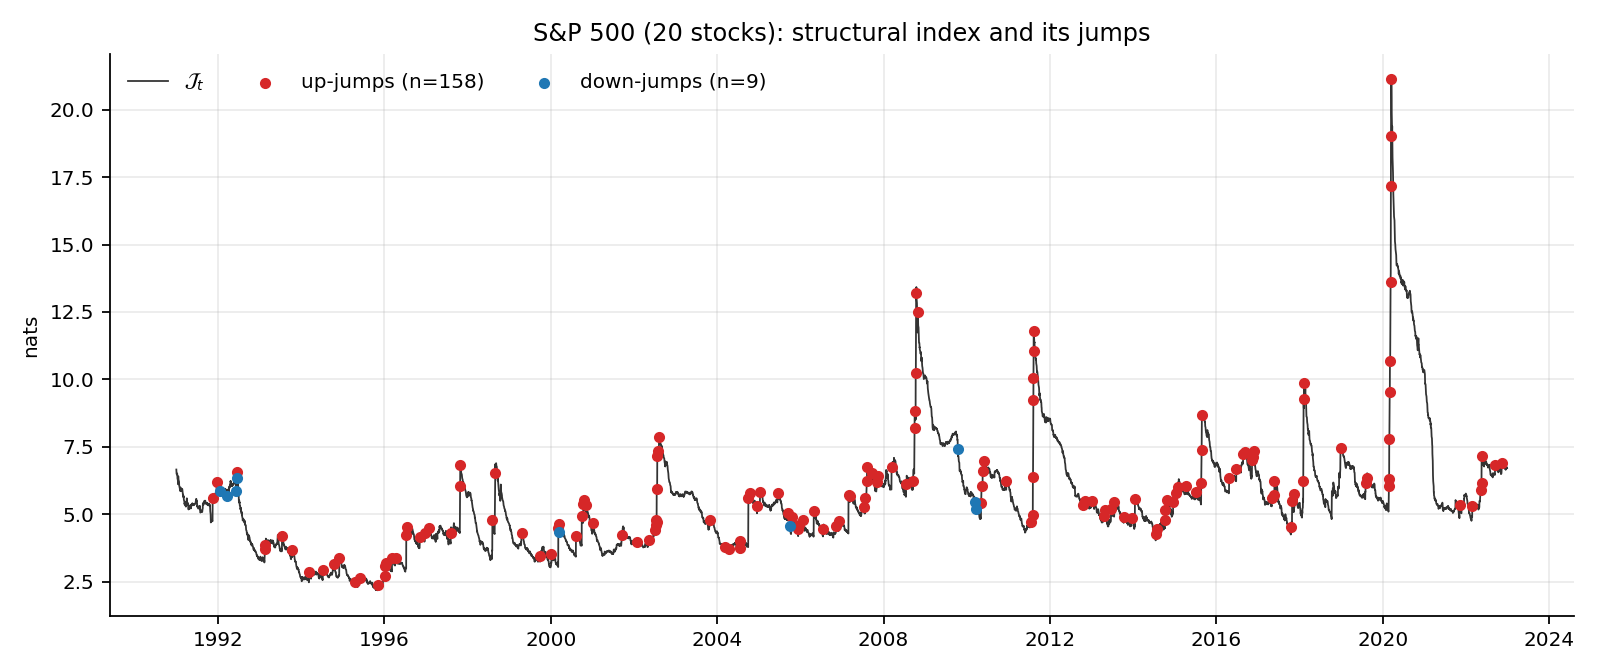
\includegraphics[width=\linewidth]{figures/sp500_structural_index_jumps.png}
\caption{L'indice structurel $\JJ_t$ sur vingt actions du S\&P~500, 1990--2022,
avec les sauts détectés. Les points rouges sont les sauts positifs, destructeurs
d'entropie, les points bleus les sauts négatifs. La dent de scie --- montée
brutale, décroissance lente --- est le contenu qualitatif de \eqref{eq:ou}.}
\label{fig:index}
\end{figure}

\begin{figure}[htbp]
\centering
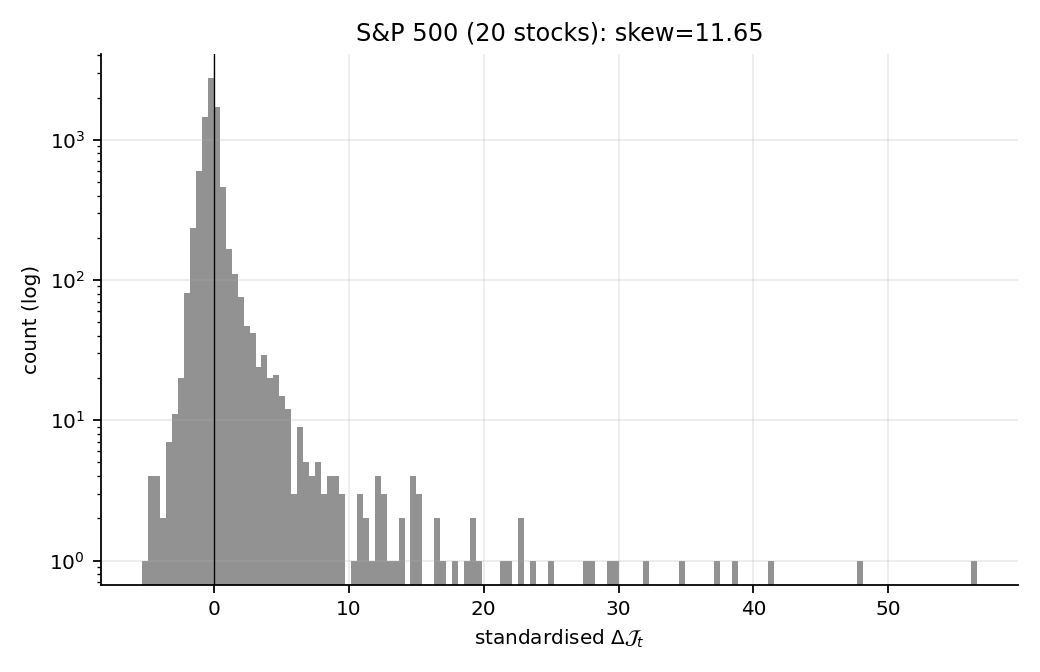
\includegraphics[width=0.62\linewidth]{figures/sp500_jump_asymmetry.png}
\caption{Distribution de $\Delta\JJ_t$ standardisé (effectifs en échelle
logarithmique). La queue droite s'étend bien au-delà de la gauche.}
\label{fig:asym}
\end{figure}

\subsection{H4 : la relaxation, face à la mémoire propre de l'estimateur}

L'estimation de \eqref{eq:ou} sur les seules dates hors saut --- afin que le
canal diffusif soit identifié sans contamination --- donne $\kappa = 0{,}0058$
par jour ($t=-3{,}75$, HAC, $p=0{,}0002$), une demi-vie de \textbf{120~jours de
bourse} et un niveau de long terme de 3,34~nats. Le panel de réplication donne
$\kappa=0{,}0050$, une demi-vie de 139~jours, $p=0{,}023$.

La demi-vie est l'endroit où les deux témoins divergent le plus nettement, et
cette divergence est instructive. Sous rééchantillonnage i.i.d., le même
estimateur renvoie $91{,}7$~jours en moyenne, de sorte que le $120{,}1$ observé
dépasse chaque réplication. Sous rééchantillonnage par blocs, il renvoie
$161{,}6$~jours, de sorte que la valeur observée tombe \emph{en dessous} de
chaque réplication. Les données se situent entre les deux témoins, et le signe de
la comparaison dépend entièrement de celui qu'on interroge. Le rééchantillonnage
par blocs concatène parfois des blocs de forte volatilité et fabrique de longues
excursions ; le rééchantillonnage i.i.d.\ brise les séries que contiennent les
marchés réels et en fabrique de courtes. Le niveau de la demi-vie n'est donc
\textbf{pas identifié}, et le chiffre de $120$~jours ne doit pas se lire comme un
temps d'absorption --- la simulation gaussienne contrôlée de la
section~\ref{sec:placebo}, où un choc unique décroît en $35$~jours sans aucune
économie, fixe le plancher de ce qui relève de la mémoire de l'estimateur.

Ce qui survit, c'est l'\emph{amplitude}. L'étendue de $\JJ$ sur l'échantillon
vaut $18{,}95$~nats contre $10{,}49$ sous le témoin i.i.d.\ et $14{,}23$ sous le
témoin par blocs, hors des quarante réplications. Son écart type franchit le
témoin i.i.d.\ ($2{,}03$ contre $1{,}61$) mais pas celui par blocs. Les marchés
réels déplacent l'indice structurel plus loin que ne le fait aucun
rééchantillonnage des mêmes rendements, ce qui est la part de P\ref{p:relax} que
les données soutiennent : non pas un taux de relaxation particulier, mais une
variable d'état qui voyage véritablement.

La figure~\ref{fig:event} ajoute une réserve que l'estimation ponctuelle masque.
En moyennant l'indice autour des sauts positifs détectés, on voit que $\JJ$
commence à monter une vingtaine de jours \emph{avant} la date signalée, culmine
environ treize jours après, et revient au niveau pré-événement au bout de
quatre-vingts jours environ. Les événements informationnels se regroupent : un
saut signalé n'est typiquement pas une arrivée isolée mais l'un des éléments
d'une séquence. L'image propre d'un saut unique suivi d'une décroissance donnée
par \eqref{eq:ou} est donc une idéalisation, et un processus d'arrivée
auto-excitant de type Hawkes s'ajusterait mieux au regroupement observé que les
arrivées poissoniennes supposées ici.

\begin{figure}[htbp]
\centering
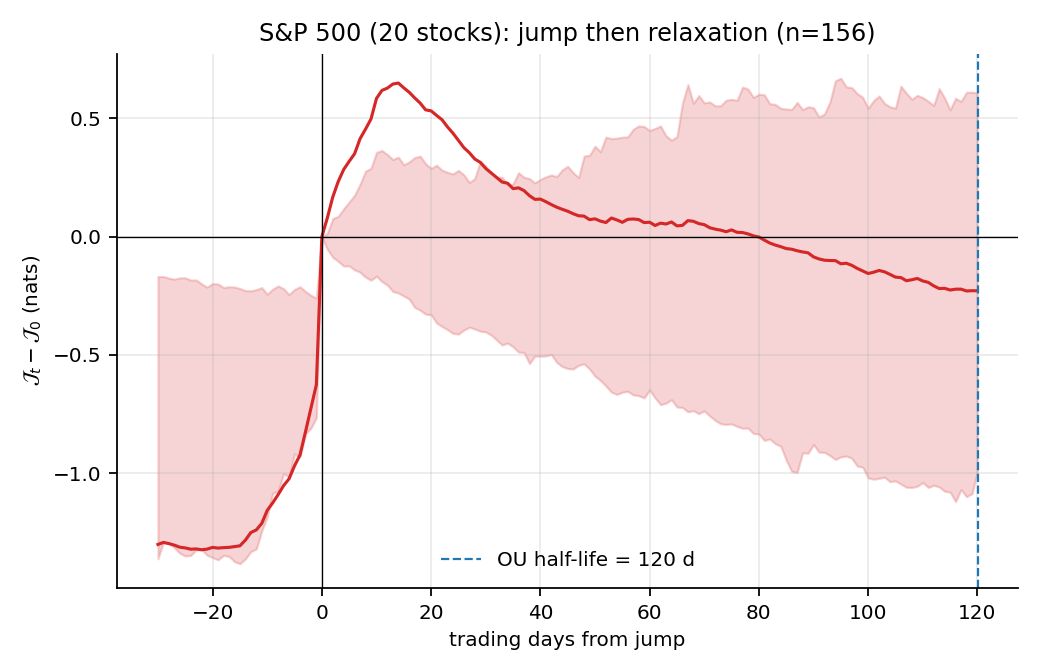
\includegraphics[width=0.62\linewidth]{figures/sp500_relaxation_event_study.png}
\caption{Trajectoire moyenne de $\JJ_t$ autour des sauts positifs détectés,
recentrée à la date de l'événement, avec la bande interquartile. La montée avant
le jour zéro est le regroupement des sauts.}
\label{fig:event}
\end{figure}

\subsection{H5 : les sauts portent un signe}

Le postulat P\ref{p:sign} prédit que les sauts positifs s'accompagnent d'une
asymétrie de marché négative. Aux dates de saut positif, la variation d'asymétrie
de marché vaut en moyenne $-0{,}052$ contre $+0{,}001$ ailleurs ; le niveau
d'asymétrie de marché à ces dates est de $-0{,}394$ contre $-0{,}214$ ; et
$\mathrm{corr}(\Delta \JJ, \Delta S_{mkt}) = -0{,}24$. Le canal d'asymétrie du
déficit monte aux dates de saut ($+0{,}010$ contre $-0{,}0002$), de même que le
co-dépassement de queue ($+0{,}008$ contre $-0{,}0002$, corrélation avec
$\Delta\JJ$ de $+0{,}35$). Le panel de réplication est plus fort sur cette
dimension : $\mathrm{corr}(\Delta\JJ,\Delta S_{mkt}) = -0{,}38$ et une variation
moyenne d'asymétrie de $-0{,}129$ aux dates de saut positif.

La réserve déjà visible au tableau~\ref{tab:h1} est que la signature d'asymétrie
est une propriété d'\emph{événement}, non de régime : trier les dates par
volatilité ne révèle aucune différence significative d'asymétrie, les trier par
saut d'entropie, si.

Face aux témoins, H5 est suggestive et rien de plus. Tous deux produisent l'effet
dans la même direction sans aucune économie, car le lien mécanique est évident
une fois énoncé : un gros rendement négatif élève simultanément $\JJ$ et abaisse
l'asymétrie mesurée de la fenêtre dans laquelle il entre. La corrélation observée
de $-0{,}243$ se situe à peu près au cinquième centile des deux témoins
($-0{,}067$ i.i.d., $-0{,}013$ blocs), et la variation moyenne d'asymétrie aux
dates de saut fait de même sous le témoin par blocs tout en restant bien à
l'intérieur du témoin i.i.d. Nous rapportons H5 comme \emph{non établie} : la
direction est la bonne, elle est cohérente sur deux témoins et deux jeux de
données (le panel de réplication donne $-0{,}38$), mais une $p$-valeur de $0{,}05$
à $0{,}10$ sur vingt réplications est une raison de chercher davantage, non un
résultat. Le postulat P\ref{p:sign} reste un postulat.

\subsection{H6 : les canaux se verrouillent sous stress}

\begin{table}[htbp]
\centering
\small
\begin{tabular}{@{}lrrr@{}}
\toprule
$\mathrm{corr}\left(-\Delta H^{dep},\,\cdot\,\right)$ & Tout & Calme & Stress \\
\midrule
S\&P~500 : avec $\Delta\DD$ (forme)      & $0{,}34$ & $0{,}04$ & $0{,}66$ \\
S\&P~500 : avec le canal de queue        & $0{,}34$ & $0{,}03$ & $0{,}68$ \\
S\&P~500 : avec le canal d'asymétrie     & $0{,}06$ & $0{,}15$ & $-0{,}01$ \\
\texttt{EuStock} : avec $\Delta\DD$      & $0{,}23$ & $0{,}05$ & $0{,}54$ \\
\bottomrule
\end{tabular}
\caption{H6 : couplage entre les deux canaux destructeurs d'entropie, par régime.}
\label{tab:h6}
\end{table}

Dans les données, le motif est frappant. En marché calme, le canal de dépendance
et le canal de queue sont effectivement sans lien ($0{,}03$) ; sous stress leur
corrélation vaut $0{,}68$. Le panel de réplication le reproduit à $0{,}05$ contre
$0{,}54$, et le couplage est porté entièrement par le canal de \emph{queue}, le
canal d'asymétrie n'y participant pas.

Les deux témoins le reproduisent aussi, et tous deux le reproduisent \emph{plus
fortement} que les données : un couplage sous stress de $0{,}90$ (i.i.d.) et
$0{,}76$ (blocs) contre le $0{,}66$ observé, et un écart stress-moins-calme de
$0{,}75$ et $0{,}67$ contre le $0{,}62$ observé. Le mécanisme est mécanique
plutôt qu'économique. Une fenêtre contenant un gros rendement commun présente à
la fois une corrélation mesurée plus élevée et des marginales mesurées plus
épaisses, de sorte que les deux canaux bougent ensemble dans toutes données où
existent de grosses journées, mélangées ou non. H6 n'est \textbf{pas soutenue}
comme preuve d'une contrainte commune contraignante.

L'ajout du témoin par blocs change toutefois l'interprétation de l'écart entre
témoin et données. Sous rééchantillonnage i.i.d., le couplage du témoin est
quasi déterministe ($0{,}90$, écart type $0{,}03$) ; préserver le regroupement
l'abaisse à $0{,}76$ avec un écart type de $0{,}07$, plus proche mais toujours
au-dessus du $0{,}66$ observé. Les vrais épisodes de stress couplent les deux
canaux \emph{moins} étroitement que l'un ou l'autre témoin. Si ce n'est pas du
bruit, cela pointe à l'opposé de la section~\ref{sec:dynamics} : dépendance et
poids de queue auraient des moteurs partiellement indépendants dans les vraies
crises, ce qu'un récit de contrainte commune ne prédit pas.

Sur l'échantillon complet, la variance de $\Delta\JJ$ se répartit à $40\%$ pour
la dépendance et $60\%$ pour la forme sur titres individuels, et à $58\%/42\%$
en sens inverse sur le panel à quatre indices --- un rappel que l'équilibre entre
canaux dépend de la coupe transversale mesurée.

\subsection{H7 : l'entropie décrit, elle ne prévoit pas}
\label{sec:h7}

\paragraph{La question, en une phrase.} Si je connais aujourd'hui l'entropie du
marché, est-ce que je sais quelque chose sur le risque des trois prochaines
semaines que la volatilité d'aujourd'hui ne me disait pas déjà ?

\paragraph{Le protocole, en quatre pas.} On compare deux modèles qui prévoient
la même chose --- la volatilité réalisée des 21~jours à venir, puis le drawdown,
puis la pire perte quotidienne. Le \emph{modèle de référence} n'utilise que le
canal d'échelle. Le \emph{modèle enrichi} y ajoute un canal d'entropie. Puis :

\begin{enumerate}
\item on estime les deux modèles sur le passé seulement, jamais sur l'avenir
qu'on cherche à prévoir ;
\item on prévoit, et on note l'erreur commise ;
\item on réestime chaque année en ajoutant l'année écoulée, et on recommence ;
\item on ne compare les erreurs que sur des dates espacées de 21~jours, pour que
deux prévisions successives ne portent pas sur les mêmes journées.
\end{enumerate}

\paragraph{Ce que \og confirmé \fg{} voudrait dire ici.} Uniquement ceci : que
le modèle enrichi commette, \emph{sur des dates qu'il n'avait pas vues au moment
d'être estimé}, des erreurs plus petites que le modèle de référence, et que
l'écart soit trop grand pour être du hasard --- ce que tranche le test de
\citet{dm1995}. Le point mérite d'être appuyé, car c'est là que la plupart des
indicateurs de ce genre se trompent eux-mêmes : \textbf{ajouter n'importe quelle
variable améliore mécaniquement l'ajustement sur les données ayant servi à
estimer le modèle}. Un bon ajustement dans l'échantillon ne prouve rien du tout.

\paragraph{Le verdict.} H7 est rejetée. Aucun canal --- ni $\JJ$, ni le déficit
$\DD$, ni le terme de dépendance, ni l'indicateur de crise, ni la part non
résorbée --- n'améliore significativement la prévision hors échantillon. La
meilleure amélioration observée, tous canaux et toutes cibles confondus, est de
$3{,}9\%$ d'erreur quadratique moyenne avec $p=0{,}52$ : indiscernable du
hasard. Plusieurs spécifications sont significativement \emph{moins bonnes} que
la référence.

Et l'illustration exacte du piège décrit plus haut : \emph{dans} l'échantillon,
les coefficients sont hautement significatifs, $p<10^{-4}$ pour $\JJ$ dans
toutes les spécifications. C'est le motif qu'on attend de fenêtres
chevauchantes, et c'est pourquoi ces chiffres ne sont pas présentés comme des
preuves.

\paragraph{Ce qu'il faut en conclure.} Que les canaux d'entropie sont
\emph{diagnostiques} et non \emph{prédictifs} : ils décrivent bien l'état
informationnel présent du marché, ils n'anticipent pas son prochain mouvement
sous une spécification linéaire. Ce résultat réplique, sur un autre jeu de
données et un protocole nettement plus exigeant, le résultat prédictif négatif
obtenu par la version antérieure de ce projet. La valeur du cadre est donc à
chercher là où la section~\ref{sec:stress} la cherche --- dans la cohérence
interne et la calibration des scénarios --- et non dans des prévisions
ponctuelles.

\subsection{Tout ceci n'est-il que de la volatilité ?}

\begin{table}[htbp]
\centering
\small
\begin{tabular}{@{}lrr@{}}
\toprule
Corrélation avec la log-volatilité glissante & S\&P~500 & \texttt{EuStock} \\
\midrule
$H^{vol}$ (canal d'échelle)          & $+0{,}56$ & $+0{,}45$ \\
$-H^{dep}$ (canal de dépendance)     & $+0{,}56$ & $+0{,}66$ \\
$\DD$ (canal de forme)               & $+0{,}09$ & $-0{,}06$ \\
$\JJ$ (indice structurel)            & $+0{,}46$ & $+0{,}60$ \\
co-dépassement de queue              & $+0{,}32$ & $+0{,}49$ \\
\bottomrule
\end{tabular}
\caption{Ce que chaque canal partage avec la volatilité.}
\label{tab:vol}
\end{table}

\begin{figure}[htbp]
\centering
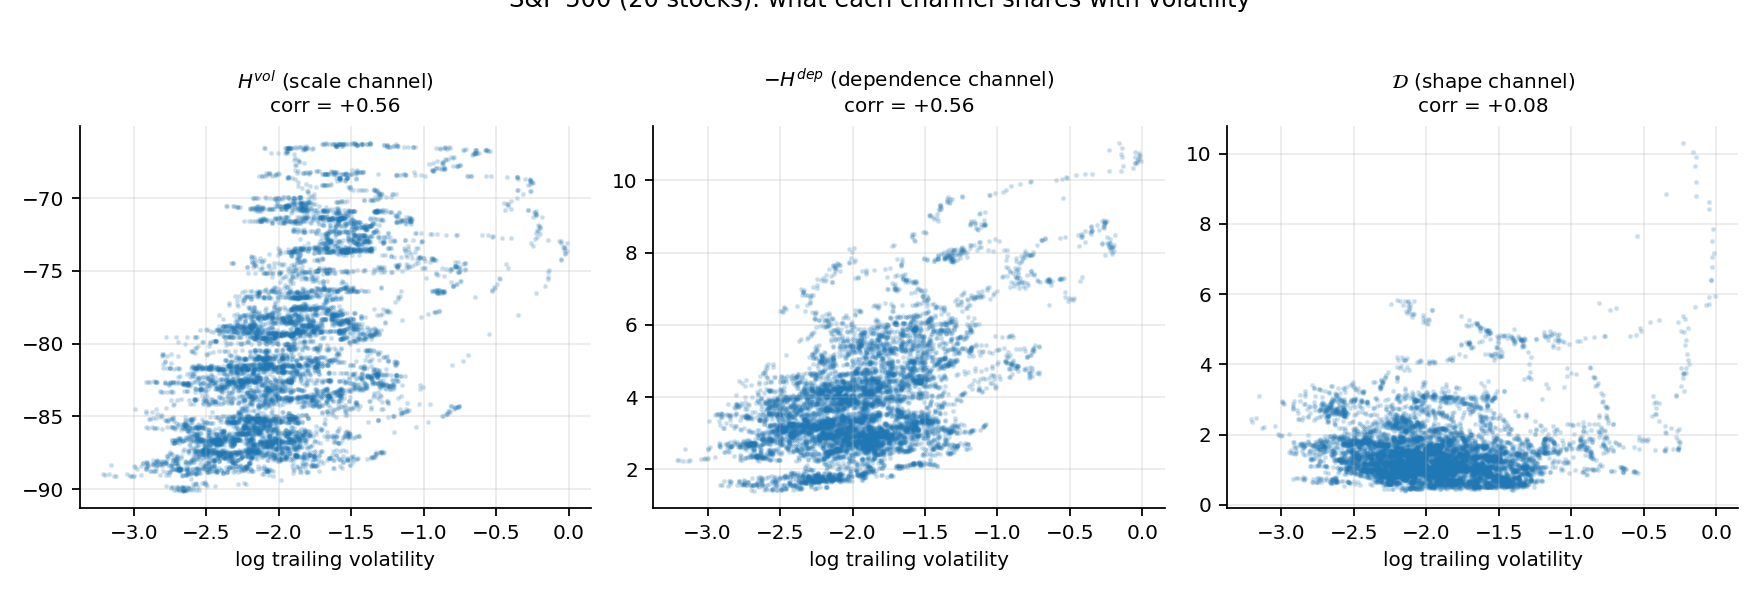
\includegraphics[width=\linewidth]{figures/sp500_channels_vs_volatility.png}
\caption{Chaque canal en fonction de la log-volatilité glissante. Les canaux
d'échelle et de dépendance la suivent ; le canal de forme, non.}
\label{fig:vol}
\end{figure}

Le tableau~\ref{tab:vol} et la figure~\ref{fig:vol} répondent à l'objection
évidente. L'indice structurel partage environ un cinquième de sa variance avec la
volatilité sur titres individuels ($r=0{,}46$) : il lui est donc lié mais loin
d'être redondant. Le canal de forme est \emph{orthogonal} à la volatilité
($r=0{,}09$ et $-0{,}06$) : l'épaisseur de queue de la distribution
conditionnelle est une dimension de l'état du marché qu'une mesure de volatilité
ne voit pas du tout. Puisque le canal de forme porte $60\%$ de la variance de
$\Delta\JJ$ sur le panel principal, l'essentiel de ce qui fait bouger l'indice
est une information que la volatilité ne contient pas.

\subsection{Réplication}

La figure~\ref{fig:eu} applique la chaîne identique aux quatre indices européens,
1991--1998. Le panel est bien trop petit pour porter seul un résultat --- quatre
actifs donnent six corrélations par paires contre 190 pour le panel principal, et
un seul cycle de stress --- mais chaque signe rapporté plus haut se reproduit :
$\JJ$ monte sous stress ($1{,}23$ contre $0{,}89$, $p<0{,}001$), les canaux se
couplent sous stress et non en marché calme ($0{,}54$ contre $0{,}05$), l'indice
relaxe avec une demi-vie de 139~jours, et les sauts positifs portent une
variation moyenne d'asymétrie de marché de $-0{,}129$ contre $+0{,}003$ ailleurs.

\begin{figure}[htbp]
\centering
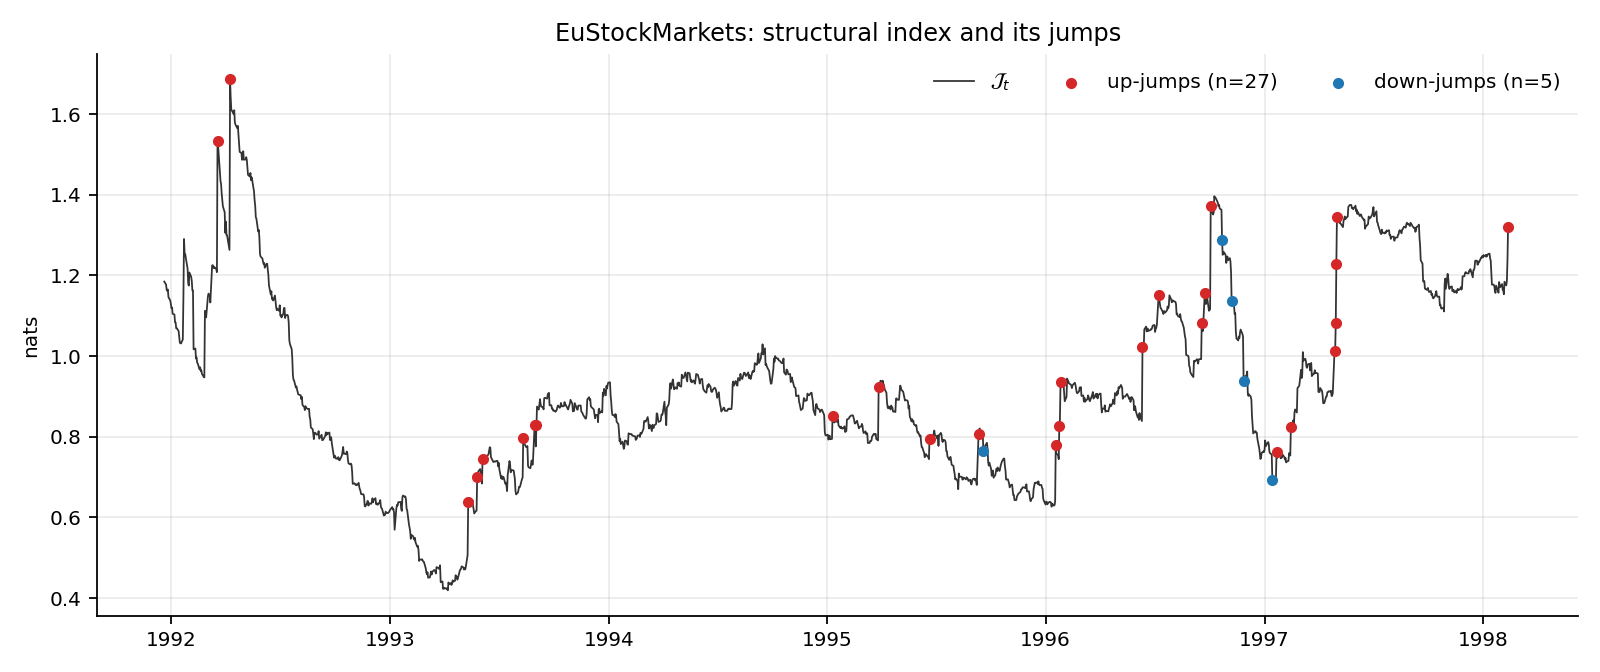
\includegraphics[width=\linewidth]{figures/eu_structural_index_jumps.png}
\caption{Réplication : l'indice structurel sur le DAX, le SMI, le CAC et le
FTSE, 1991--1998. Les hausses visibles coïncident avec les épisodes du SME de
septembre 1992 et 1993 et avec la crise asiatique d'octobre--novembre 1997.}
\label{fig:eu}
\end{figure}

\section{Tests de résistance par l'entropie}
\label{sec:stress}

\subsection{La construction}

\begin{definition}[Scénario en boule d'entropie]
Étant donné la distribution conditionnelle d'aujourd'hui $p_0$ et une sévérité
$\eta>0$, le scénario de sévérité $\eta$ pour une fonctionnelle de risque $\rho$
est
\begin{equation}
\label{eq:ball}
p^\star_\eta \;=\; \arg\max_{p\,:\,\KL{p}{p_0}\,\le\,\eta} \rho(p).
\end{equation}
\end{definition}

Pour un portefeuille linéaire et une référence gaussienne, seule la projection
unidimensionnelle importe. Avec $m_0,s_0$ la moyenne et l'écart type du
portefeuille et $u=(m-m_0)/s_0$, $v=s/s_0$, la contrainte est
$g(u,v)=\tfrac12\!\left(u^2+v^2-1-2\log v\right)\le\eta$, et pour tout $\rho$ de
la forme $-m+cs$ --- la VaR gaussienne et l'expected shortfall en sont toutes deux
--- la solution vérifie $u=-t$, $v-v^{-1}=ct$, où $t$ est fixé par $g=\eta$. Le
cas particulier $c=0$ est le contrôle de cohérence à retenir :

\begin{equation}
\text{un scénario purement directionnel de }\eta\text{ nats est exactement un mouvement de }\sqrt{2\eta}\text{ sigmas.}
\end{equation}

Un nat achète $1{,}41$~sigma. C'est le taux de change entre information et
risque, et c'est toute la raison pour laquelle la construction est utilisable par
un comité : le paramètre de sévérité n'est pas une abstraction.

\subsection{Calibrer le rayon}

Le rayon n'est pas ici un choix de modélisation. Définissons le flux
d'information à $h$ pas
\begin{equation}
I^{(h)}_t \;=\; \KL{p_t}{p_{t-h}},
\end{equation}
la divergence entre la distribution conditionnelle du marché aujourd'hui et celle
d'il y a $h$ jours --- de combien le marché a révisé sa propre vue. C'est une
divergence en bonne et due forme entre deux lois conditionnelles de rendements,
mesurée dans la même unité que le rayon du scénario, ce qui rend la calibration
cohérente. Les quantiles de $I^{(21)}$, amincis en blocs non chevauchants,
convertissent une période de retour en rayon.

\begin{table}[htbp]
\centering
\small
\begin{tabular}{@{}lrrrrrr@{}}
\toprule
Période de retour & 1~an & 2~ans & 5~ans & 10~ans & 20~ans & 50~ans$^\dagger$ \\
\midrule
rayon $\eta$ (nats)             & 1,04 & 1,63 & 2,34 & 3,88 & 7,54 & 13,16 \\
choc directionnel ($\sigma$)    & $-0{,}58$ & $-0{,}72$ & $-0{,}84$ & $-1{,}06$ & $-1{,}45$ & $-1{,}88$ \\
multiplicateur de volatilité    & 2,04 & 2,33 & 2,63 & 3,15 & 4,10 & 5,20 \\
volatilité annualisée du portef.\ & $41\%$ & $47\%$ & $53\%$ & $63\%$ & $82\%$ & $105\%$ \\
ES$_{99}$ à un jour             & $7{,}6\%$ & $8{,}8\%$ & $9{,}9\%$ & $12{,}0\%$ & $15{,}6\%$ & $19{,}9\%$ \\
\bottomrule
\end{tabular}
\caption{Échelle de sévérité pour un portefeuille équipondéré des vingt titres,
calibrée sur 383 observations non chevauchantes de flux d'information à
21~jours. La référence d'aujourd'hui est une volatilité annualisée de $20\%$ et
une ES$_{99}$ à un jour de $3{,}4\%$. $^\dagger$ au-delà de l'échantillon :
l'échelon cinquantennal exige un quantile que 33~ans d'historique ne peuvent pas
résoudre et constitue une extrapolation de la queue empirique.}
\label{tab:ladder}
\end{table}

Deux traits du tableau~\ref{tab:ladder} méritent une lecture attentive. Le
scénario dépense son budget surtout en \emph{variance} plutôt qu'en direction ---
à l'échelon annuel, un doublement de la volatilité et seulement un choc de
dérive de $0{,}58\sigma$ --- parce que l'expected shortfall est plus sensible à
l'échelle qu'à la position. Et le rayon n'est pas comparable d'un univers à
l'autre : une divergence KL croît avec la dimension du vecteur de rendements, de
sorte que l'échelle du panel à quatre indices va de $0{,}09$ à $0{,}21$~nat là où
celle des vingt titres va de $1{,}04$ à $13{,}2$. Une échelle doit être calibrée
pour le portefeuille auquel elle s'appliquera.

\begin{figure}[htbp]
\centering
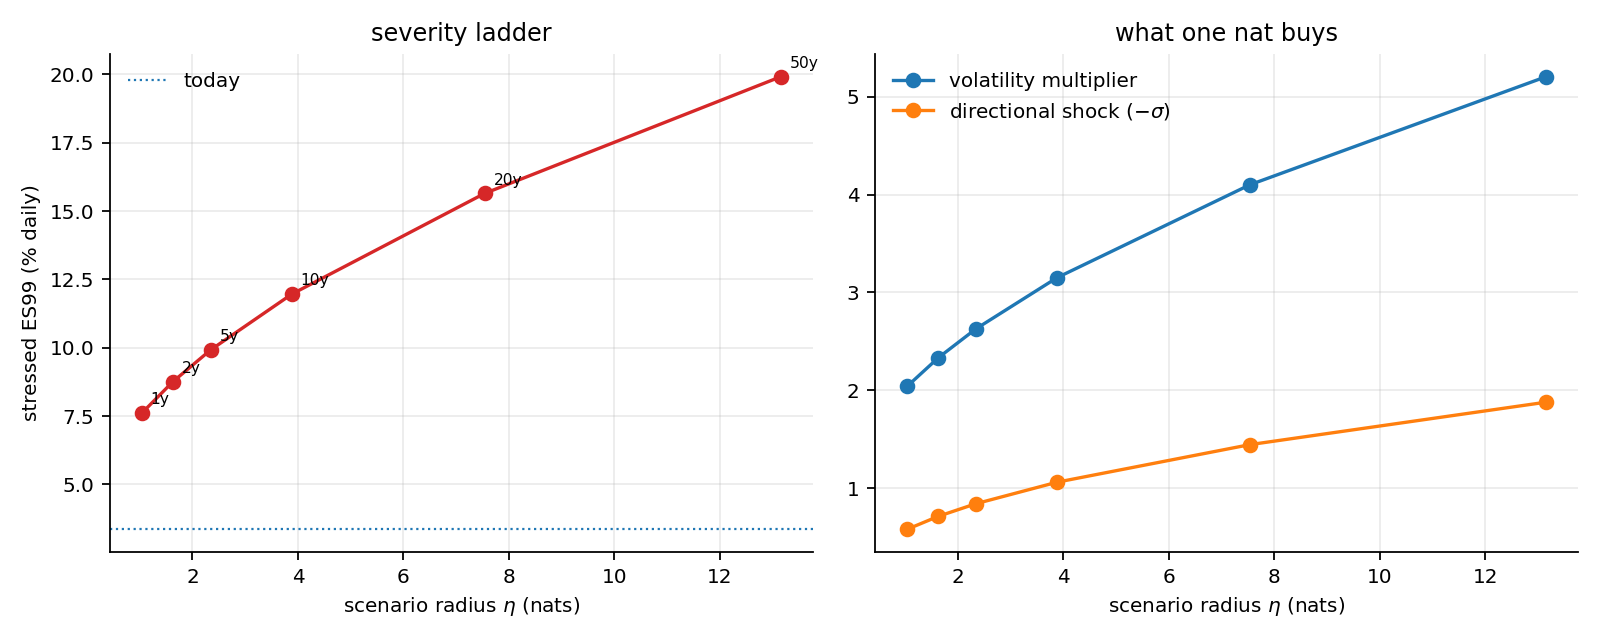
\includegraphics[width=\linewidth]{figures/sp500_stress_ladder.png}
\caption{À gauche : ES$_{99}$ à un jour sous stress en fonction du rayon du
scénario, périodes de retour indiquées. À droite : ce qu'achète un nat, réparti
entre le multiplicateur de volatilité et le choc directionnel.}
\label{fig:ladder}
\end{figure}

\subsection{Ce que cela apporte face aux tests de résistance en volatilité, moyenne et asymétrie}

La comparaison n'est pas rhétorique, car la même métrique tarife un scénario
classique. Prenons la distribution conditionnelle d'aujourd'hui et construisons
le bundle des manuels : volatilités marginales multipliées, toutes les
corrélations par paires forcées à un même nombre élevé, un choc directionnel de
plusieurs sigmas. Son prix informationnel est
$\KL{p_{\text{classique}}}{p_0}$, calculable en forme fermée.

\begin{table}[htbp]
\centering
\small
\begin{tabular}{@{}lrrr@{}}
\toprule
Bundle classique & modéré & standard & sévère \\
\midrule
multiplicateur de volatilité       & $1{,}5$ & $2{,}0$ & $3{,}0$ \\
toutes corrélations forcées à      & $0{,}70$ & $0{,}90$ & $0{,}95$ \\
choc directionnel                  & $-2\sigma$ & $-3\sigma$ & $-4\sigma$ \\
\midrule
ES$_{99}$ à un jour impliquée      & $9{,}1\%$ & $13{,}7\%$ & $20{,}3\%$ \\
prix informationnel (nats)         & $6{,}80$ & $9{,}97$ & $20{,}19$ \\
\quad dont : composante directionnelle & $2{,}00$ & $4{,}50$ & $8{,}00$ \\
\quad \phantom{dont :} composante volatilité & $4{,}39$ & $16{,}14$ & $58{,}03$ \\
\quad \phantom{dont :} composante corrélation & $2{,}43$ & $8{,}10$ & $13{,}50$ \\
période de retour impliquée        & $\sim11$~ans & $>30$~ans & hors échantillon \\
\midrule
\textbf{scénario entropique à même ES$_{99}$} & $\mathbf{1{,}85}$ & $\mathbf{5{,}47}$ & $\mathbf{13{,}74}$ \\
\quad sa période de retour         & $2{,}3$~ans & $10{,}6$~ans & $\sim32$~ans \\
\quad surcoût informationnel       & $73\%$ & $45\%$ & $32\%$ \\
\bottomrule
\end{tabular}
\caption{Tarification des bundles de stress des manuels face au flux
d'information propre au marché, et comparaison de chacun avec le scénario
entropique délivrant la même expected shortfall. Échelons de référence du
tableau~\ref{tab:ladder} : le scénario vicennal vaut $7{,}54$~nats, le
cinquantennal $13{,}16$ ; la pire journée unique en 33~ans se tarife à $9{,}03$.}
\label{tab:classical}
\end{table}

Le tableau~\ref{tab:classical} est le point appliqué de l'article, et il dit
quelque chose de plus tranchant que \og les scénarios classiques sont trop
sévères \fg{}. Le bundle standard coûte $9{,}97$~nats, ce qui le situe entre les
échelons vicennal et cinquantennal --- une sévérité défendable pour un test de
résistance réglementaire, et que personne autour de la table n'avait le moyen de
savoir avoir choisie. Ce qui n'est pas défendable, c'est l'efficience. Un
scénario entropique délivre la même expected shortfall de $13{,}7\%$ pour
$5{,}47$~nats. Le comité croit avoir spécifié quelque chose de l'ordre d'un
événement trentennal ; mesuré par la perte qu'il produit réellement, il a
spécifié un événement décennal et payé une invraisemblance trentennale. Le bundle
modéré est pire : il se tarife comme un événement de onze ans et délivre une
perte \emph{biennale}, un surcoût de $73\%$.

Où passe l'argent ? La composante directionnelle est bon marché et exactement
tarifée : déplacer la moyenne du portefeuille de $k$ écarts types coûte
$k^2/2$~nats, soit $4{,}5$ pour trois sigmas. La composante chère est le
doublement uniforme de chaque volatilité marginale, à $16{,}1$~nats à elle seule
--- davantage que le bundle entier. Forcer toutes les corrélations à $0{,}9$ coûte
$8{,}1$~nats à elle seule.

Les composantes ne sont pas additives, et la façon dont elles ne le sont pas est
instructive : les trois somment à $28{,}7$~nats alors que le bundle en coûte
$9{,}97$. Forcer les corrélations à la hausse effondre la covariance sur un
sous-espace de rang quasi un auquel la distribution de référence accorde déjà une
variance généreuse --- le mode de marché --- de sorte que mettre à l'échelle cette
structure effondrée est bien moins coûteux que mettre à l'échelle la structure de
rang plein ($\mathrm{tr}(\Sigma_0^{-1}\Sigma_1)$ tombe de $20$ à $10{,}5$ quand
les corrélations sont forcées, avant même que le multiplicateur de volatilité ne
soit appliqué). Le choc de volatilité et le choc de corrélation se paient
partiellement l'un l'autre.

C'est exactement la structure qu'a identifiée H6 dans les données. Les vraies
crises n'égalisent pas les corrélations et ne gonflent pas toutes les volatilités
indépendamment ; elles chargent la coupe transversale sur un ou deux modes
collectifs et épaississent conjointement les queues des marginales. Un cadre qui
choque volatilité, corrélation et forme comme trois scalaires séparés n'a aucun
moyen de représenter cela, ni aucun moyen de s'apercevoir que son bundle achète
la sévérité avec une marge de $30$ à $70\%$.

Quatre avantages concrets sur l'approche volatilité/moyenne/asymétrie en
découlent.

\begin{enumerate}
\item \textbf{Une échelle de sévérité unique, dans une unité qui ne dépend pas de
l'actif.} Les scénarios deviennent comparables entre desks, portefeuilles et
classes d'actifs, et la sévérité se cite avec une période de retour plutôt
qu'avec un adjectif.
\item \textbf{Cohérence interne par construction.} Les chocs de position et
d'échelle proviennent d'un même budget et d'une même optimisation. Un bundle qui
choque volatilité, corrélation et asymétrie indépendamment peut décrire, et
décrit souvent, une distribution que le marché ne saurait produire.
\item \textbf{Les scénarios existants peuvent être audités plutôt que
remplacés.} Tout gabarit réglementaire ou jugement de comité reçoit un prix en
nats et une période de retour, de sorte que la question de savoir si un test de
résistance est calibré devient arithmétique. C'est le bénéfice pratique du
tableau~\ref{tab:classical}.
\item \textbf{Le test de résistance inversé est offert.} Au lieu de demander ce
que fait un scénario, on demande quel est le scénario le moins cher produisant
une perte donnée. Sur le panel principal, la perte quotidienne empirique à
$99\%$ ($3{,}2\%$) coûte $1{,}5$~nat ; celle à $99{,}9\%$ ($7{,}7\%$) coûte
$4{,}8$ ; la pire journée en 33~ans ($11{,}5\%$) coûte $9{,}0$. Lire ces chiffres
au regard du tableau~\ref{tab:ladder} convertit en fréquence une perte qui
préoccupe le conseil.
\end{enumerate}

Une mise en garde sur le quatrième point. Les tests de résistance inversés
calculés de façon non paramétrique, en inclinant l'échantillon empirique,
dégénèrent à mesure que le rayon croît : à $9{,}0$~nats, la mesure inclinée a une
taille d'échantillon effective de $1{,}0$, c'est-à-dire qu'elle est la pire
journée unique déguisée en distribution. L'implémentation rapporte la taille
d'échantillon effective précisément pour cette raison, et la construction en
boule gaussienne devrait être employée dès qu'elle tombe sous quelques dizaines.

\subsection{Deux indicateurs de suivi}

La séparation saut/diffusion livre deux quantités productibles quotidiennement à
coût négligeable. L'indicateur de \emph{crise} est la composante de saut positif
standardisée de $\JJ$ : quelle quantité d'information est arrivée aujourd'hui, en
unités de l'échelle diffusive locale, nulle lorsqu'aucun saut n'est détecté.
L'indicateur de \emph{part non résorbée} est $\JJ_t$ rapporté à son maximum
glissant : quelle part de ce qui est déjà arrivé ne s'est pas encore relâchée.
Sous P\ref{p:relax}, il devrait décroître avec une demi-vie $\ln2/\kappa$ ; un
marché où il reste proche de un sensiblement plus longtemps est un marché où le
choc n'a pas été absorbé. Ni l'un ni l'autre n'améliore une prévision de
volatilité (H7) ; tous deux décrivent un état que la volatilité ne décrit pas.

\subsection{Pertinence pour la solvabilité en assurance}

Trois points relient ceci au volet assurance du projet d'ensemble. D'abord, un
scénario en boule d'entropie est un objet naturel pour l'ORSA : il produit une
distribution stressée complète, non un vecteur de chocs, de sorte qu'il alimente
directement un calcul de capital et porte un énoncé de plausibilité défendable.
Ensuite, la décomposition en composantes du tableau~\ref{tab:classical} concerne
la formule standard de Solvabilité~II, dont le crédit de diversification est bâti
sur une matrice de corrélation fixe : choquer volatilités et corrélations comme
des scalaires séparés, ce qui est l'ajustement conservateur usuel, achète une
perte de queue donnée avec une marge de $30$ à $70\%$ en termes de plausibilité,
parce que cela ne représente pas la façon dont les crises observées
redistribuent la dépendance --- sur quelques modes collectifs plutôt
qu'uniformément. Enfin, les propriétés de cohérence des mesures de risque
entropiques \citep{ahmadijavid2012,artzner1999} rendent le cadre $\JJ$ compatible
en principe avec des exigences de capital en modèle interne, bien que rien ici
n'ait été testé sur des portefeuilles de passifs et que les panels courts et à
basse fréquence typiques des données d'assurance mettraient à mal chacun des
estimateurs employés plus haut.

\section{Limites}
\label{sec:limits}

\paragraph{Le pont est un argument, pas une preuve.} La
section~\ref{sec:bridge-caveats} liste les défaillances de l'impact linéaire et
de l'échangeabilité des signes. Rien d'empirique ci-dessous ne dépend de
l'horloge de volume, mais le cadrage, si.

\paragraph{Le déficit est estimé marginalement.} Le canal de forme capture la
non-gaussianité marginale et la dépendance de copule gaussienne ; la dépendance
de queue non linéaire est mesurée séparément plutôt qu'intégrée, de sorte que
$\JJ$ sous-estime la divergence véritable, d'un montant lui-même maximal sous
stress.

\paragraph{Le témoin mécanique avale une hypothèse entière.} L'asymétrie des
sauts est intégralement reproduite par des données i.i.d.\ de même loi marginale,
et environ les deux tiers de la relaxation mesurée relèvent de la mémoire de
l'estimateur. Les résultats de persistance et d'amplitude survivent ; le résultat
d'asymétrie, non, et aucun lecteur ne devrait citer le chiffre de 158~contre~9
sans le témoin à côté. Vingt réplications, c'est aussi peu : les quantiles du
témoin au tableau~\ref{tab:placebo} sont eux-mêmes estimés avec une erreur
visible, et une centaine de réplications affinerait les $p$-valeurs qui se
situent actuellement à $0{,}05$.

\paragraph{Les arrivées poissoniennes sont le mauvais modèle.} La
figure~\ref{fig:event} montre un regroupement que \eqref{eq:ou} n'accommode pas.
Un processus d'arrivée auto-excitant de Hawkes est la spécification suivante
évidente.

\paragraph{Vingt titres, c'est une petite coupe transversale.} Le canal de
dépendance est sensible à $N$, l'équilibre entre canaux se déplace avec lui, et
le rayon KL n'est pas comparable d'un univers à l'autre. Les résultats devraient
être reproduits sur une large coupe transversale --- le fichier sectoriel de
Kenneth French, ou CRSP --- avant qu'aucun chiffre présenté ici ne soit traité
comme une constante de la nature.

\paragraph{L'échelle de sévérité extrapole en queue.} Avec 383 observations non
chevauchantes de flux d'information, les échelons au-delà d'une vingtaine
d'années sont des interpolations de la queue empirique, non des mesures. Ajuster
une queue de Pareto généralisée à $I^{(h)}$ serait la correction disciplinée.

\paragraph{Rien ici ne prévoit.} H7 est rejetée sur deux jeux de données sous un
protocole exigeant. Tout usage de ces mesures devrait être diagnostique.

\section{Conclusion}

La contribution théorique est une chaîne explicite sur ce qui, en chaque maillon,
relève du théorème et ce qui relève de l'hypothèse. Le maximum d'entropie sous
contraintes de moments d'ordre un et deux donne une gaussienne ; appliqué en
temps-volume, le volume échangé fournissant le budget de variance, il donne des
rendements gaussiens conditionnels au volume, et la cohérence temporelle en fait
un mouvement brownien subordonné puis un prix brownien géométrique. Lu à
l'envers, des prix non gaussiens mesurent la distance à l'ignorance maximale, et
cette distance se décompose en un canal de dépendance et un canal de forme dont
la somme, l'indice structurel $\JJ$, est sans échelle et positive. Conditionner
ne peut pas augmenter l'entropie espérée, donc l'entropie chute par sauts dont la
taille \emph{espérée} est l'information mutuelle de la nouvelle ; que cette entropie se rétablisse
par diffusion, et que la chute soit unilatérale dans la direction des pertes,
sont les deux postulats que l'article ajoute et teste.

Le tableau empirique est surtout un avertissement, et nous pensons que c'est là
le résultat utile. Chaque affirmation descriptive du cadre est visible dans les
données : le stress élève l'indice structurel, l'indice est en dents de scie, les
sauts sont unilatéraux, ils portent une asymétrie négative, et les canaux de
dépendance et de queue se couplent sous stress. Passé par un témoin qui conserve
la loi marginale et brouille la chronologie, l'essentiel disparaît --- et
plusieurs statistiques ressortent \emph{plus grandes} dans les données mélangées
que dans les données réelles. Une fonctionnelle convexe positive de moments
estimés d'ordre deux, trois et quatre monte brutalement et redescend en douceur
dès qu'une observation à queue épaisse entre dans l'estimateur, et elle le fait
que l'information arrive ou non par paquets. Cette mise en garde vaut pour tout
indicateur de crise fondé sur l'entropie, et pas seulement pour celui-ci, et nous
ne l'avons pas trouvée énoncée dans la littérature appliquée.

Exactement deux statistiques franchissent les deux témoins, et ce sont les deux
qu'il faut retenir. Ce qui sépare une crise d'une série de gros rendements, c'est
que la coupe transversale se couple : le signal de régime du canal de dépendance
vaut entre trois et six fois celui des témoins, tandis que celui du canal de
forme est inférieur aux deux. Et l'indice structurel voyage plus loin sur
l'échantillon que dans tout rééchantillonnage des mêmes rendements. Le taux de
relaxation lui-même n'est pas identifié --- il se situe entre les deux témoins ---
de sorte que P1 est soutenu par l'amplitude et non par une demi-vie. Deux autres
résultats vont à l'encontre de l'intérêt de l'article : la compensation
volatilité--dépendance obtenue sur portefeuilles sectoriels ne survit pas au
passage aux titres individuels, et aucun canal d'entropie ne prévoit quoi que ce
soit hors échantillon.

La contribution appliquée est ce que le cadre apporte une fois qu'on cesse de lui
demander de prévoir. Mesurer la sévérité d'un scénario en nats donne au test de
résistance une unité ; calibrer cette unité sur le flux d'information réalisé du
marché lui donne une fréquence ; et résoudre pour la pire distribution dans la
boule qui en résulte donne un scénario qui ne peut pas être incohérent en
interne. Appliqué à l'envers, il tarife les scénarios que les institutions font
déjà tourner : sur cet échantillon, un bundle standard des manuels se situe entre
les échelons vicennal et cinquantennal mais achète sa perte de queue avec une
marge de $45\%$, parce qu'il dépense l'essentiel de son budget à gonfler
uniformément chaque volatilité marginale --- ce qui n'est pas la voie que
prennent les crises observées.


\appendix

\section{Unités, invariance, et ce qui est calculable}
\label{app:units}

\paragraph{Le nat.} L'entropie $H=-\sum_i p_i\log p_i$ n'est définie qu'une fois
la base du logarithme choisie, et ce choix \emph{est} le choix de l'unité. Avec
$\log_2$ on obtient des bits (shannons), avec $\log_{10}$ des dits, et avec le
logarithme népérien des \emph{nats}. Un nat est l'information apportée par une
observation qui divise l'espace des possibles par $e\approx2{,}718$, là où un bit
le divise par deux. La conversion est
$1~\text{nat}=1/\log 2\approx1{,}4427$~bit. Tout ce papier emploie le logarithme
népérien : entropies, déficits, divergences, rayons de scénario et indice
structurel sont en nats.

Trois lectures opérationnelles, de la plus utile à la plus abstraite. D'abord le
taux de change établi en section~\ref{sec:stress} : un scénario purement
directionnel de $\eta$ nats est un mouvement de $\sqrt{2\eta}$ sigmas, donc
$k$~sigmas coûtent $k^2/2$ nats. Ensuite le codage : $\KL{p}{q}$ nats est
l'excès de longueur de code attendu lorsqu'on encode des données de loi $p$ avec
un code optimal pour $q$. Enfin le test d'hypothèse : une divergence de un nat
par observation signifie que le rapport de vraisemblance en faveur de $p$ croît
en moyenne d'un facteur $e$ à chaque observation.

\paragraph{$h$ dépend des unités, les divergences non.} L'entropie différentielle
d'une variable continue vérifie, pour toute transformation affine inversible,
\begin{equation}
\label{eq:h-scaling}
h(aX+b) \;=\; h(X) + \log|a| ,
\qquad\text{et en dimension } N,\quad h(AX+b)=h(X)+\log|\det A| .
\end{equation}
Exprimer les rendements en pourcentages plutôt qu'en décimales ajoute donc
$N\log 100$ à $h$ : le \emph{niveau} de $h$, et par conséquent celui de
$H^{vol}$ et de $H^{cov}$, n'a aucune valeur absolue interprétable. En revanche
$\KL{p}{q}$, $I(X;Y)$, $\DD$ et $\JJ$ sont invariants par tout changement de
variable inversible, les jacobiens se simplifiant entre numérateur et
dénominateur du logarithme. \emph{Un chiffre en nats n'est comparable d'un jeu
de données à l'autre que si c'est une divergence.} C'est la raison structurelle
pour laquelle l'article construit un indice sans échelle.

\paragraph{Comment calcule-t-on $h(X)$ ?} Dans le cas gaussien, en forme fermée
(annexe~\ref{app:gauss}). Dans le cas général, on ne le peut pas sans connaître
$p$. Des estimateurs non paramétriques existent --- espacements de
\citet{vasicek1976}, plus proches voisins de Kozachenko--Leonenko, méthodes à
noyau --- mais tous se dégradent rapidement au-delà de trois ou quatre
dimensions. Estimer une entropie différentielle en dimension~20 sur une fenêtre
de 252~jours est hors de portée.

L'article ne calcule donc \emph{jamais} $h(p)$. Il calcule $h(q)$ en forme
fermée à partir de $\widehat\Sigma$, et le déficit $\DD$ par une approximation
de la \emph{différence} d'entropies marginales. Une différence d'entropies est
sans dimension et estimable ; une entropie différentielle nue ne l'est pas.
Toute l'architecture --- décomposer plutôt qu'estimer directement --- découle de
cette contrainte.

\section{Entropie gaussienne : démonstration de l'équation~\eqref{eq:ceiling}}
\label{app:gauss}

\begin{proof}[Étape A : entropie d'une gaussienne multivariée]
Pour $q=\mathcal N(\mu,\Sigma)$ sur $\mathbb{R}^N$,
\[
\log q(x) = -\tfrac12\left[N\log 2\pi + \log\det\Sigma + (x-\mu)'\Sigma^{-1}(x-\mu)\right],
\]
donc
\[
h(q) = -\mathbb{E}_q[\log q] = \tfrac12 N\log 2\pi + \tfrac12\log\det\Sigma
+ \tfrac12\,\mathbb{E}\!\left[(X-\mu)'\Sigma^{-1}(X-\mu)\right].
\]
La dernière espérance se calcule par l'astuce de la trace : un scalaire égale sa
trace, et la trace est cyclique, d'où
\[
\mathbb{E}\!\left[(X-\mu)'\Sigma^{-1}(X-\mu)\right]
= \mathbb{E}\!\left[\operatorname{tr}\!\left(\Sigma^{-1}(X-\mu)(X-\mu)'\right)\right]
= \operatorname{tr}(\Sigma^{-1}\Sigma) = \operatorname{tr}(I_N) = N .
\]
En regroupant, $h(q)=\tfrac12\left[N\log2\pi+\log\det\Sigma+N\right]
=\tfrac12\log\!\left((2\pi e)^N\det\Sigma\right)$.
\end{proof}

\begin{proof}[Étape B : factorisation du déterminant]
Avec $\Sigma=DRD$, $D=\operatorname{diag}(\sigma_1,\dots,\sigma_N)$ et $R$ la
matrice de corrélation, la multiplicativité du déterminant donne
$\det\Sigma=\det(D)\det(R)\det(D)=\left(\prod_i\sigma_i\right)^2\det R$.
\end{proof}

\begin{proof}[Étape C : substitution]
$\tfrac12\log\det\Sigma
=\tfrac12\log\!\left[\left(\prod_i\sigma_i\right)^2\det R\right]
=\sum_i\log\sigma_i+\tfrac12\log\det R$, d'où
$h(q)=\tfrac N2\log(2\pi e)+\sum_i\log\sigma_i+\tfrac12\log\det R$, qui est
l'équation~\eqref{eq:ceiling}.
\end{proof}

\paragraph{Signe du canal de dépendance.} L'inégalité de Hadamard donne
$\det R\le\prod_i R_{ii}=1$ pour une matrice semi-définie positive. Une
démonstration plus parlante passe par le spectre : $\det R=\prod_k\lambda_k$
avec $\sum_k\lambda_k=\operatorname{tr}R=N$, et l'inégalité arithmético-géométrique
donne $\prod_k\lambda_k\le\left(\sum_k\lambda_k/N\right)^N=1$, avec égalité si
et seulement si toutes les valeurs propres valent~1, c'est-à-dire $R=I$. Donc
$H^{dep}\le0$ : \emph{la corrélation détruit toujours de l'entropie}.

Dans le cas bivarié, $\det R=1-\rho^2$ et $H^{dep}=\tfrac12\log(1-\rho^2)$ ; pour
$\rho=0{,}9$ cela vaut $-0{,}83$~nat. Remarquons que $-H^{dep}$ est alors
exactement l'information mutuelle entre les deux actifs : la corrélation est de
l'information partagée, donc de l'entropie détruite.

\paragraph{Note de lecture sur les tableaux.} Les colonnes $H^{cov}$ des
tableaux~\ref{tab:h1} et suivants rapportent $H^{vol}+H^{dep}$ et
\textbf{omettent la constante} $\tfrac N2\log(2\pi e)$, qui vaut $28{,}38$~nats
pour $N=20$. Ce décalage constant est sans conséquence puisque seules les
différences entre régimes et les variations temporelles sont interprétées, mais
il explique que les niveaux rapportés soient négatifs.

\section{Le déficit d'entropie : pourquoi $\DD=h(q)-h(p)$}
\label{app:deficit}

La divergence de Kullback--Leibler entre une loi $p$ et une loi de référence $q$
est $\KL{p}{q}=\int p\log(p/q)$, positive et nulle si et seulement si $p=q$
presque partout. Elle n'est ni symétrique ni munie d'une inégalité triangulaire :
ce n'est pas une distance, d'où le terme de divergence. Les lettres \og KL \fg{}
sont les initiales de Kullback et Leibler.

\begin{proposition}
\label{prop:deficit}
Si $q=\mathcal N(\mu,\Sigma)$ a \emph{les deux premiers moments de $p$}, alors
$\KL{p}{q}=h(q)-h(p)$.
\end{proposition}

\begin{proof}
$\KL{p}{q}=-h(p)-\mathbb{E}_p[\log q(X)]$. Or $\log q$ est exactement
quadratique en $x$, donc son espérance ne dépend que de la moyenne et de la
covariance de la loi sous laquelle on l'évalue. Comme $p$ et $q$ partagent ces
deux moments,
$\mathbb{E}_p\!\left[(X-\mu)'\Sigma^{-1}(X-\mu)\right]=\operatorname{tr}(\Sigma^{-1}\Sigma)=N
=\mathbb{E}_q[\cdot]$, d'où $\mathbb{E}_p[\log q]=\mathbb{E}_q[\log q]=-h(q)$ et
donc $\KL{p}{q}=h(q)-h(p)$.
\end{proof}

L'hypothèse de coïncidence des moments est essentielle : sans elle l'identité
tombe. C'est tout le contenu de la proposition~\ref{prop:maxent}, lue comme une
mesure plutôt que comme un théorème d'existence. Économiquement, $\DD$ est le
prix en nats du mensonge \og le marché est gaussien \fg{} : l'incertitude
apparente que la description gaussienne surestime, parce que la loi véritable est
plus concentrée que ne le laisse croire sa seule covariance.

\section{L'indice structurel est une divergence}
\label{app:index}

\begin{proposition}
\label{prop:index}
Avec $q_i=\mathcal N(\mu_i,\sigma_i^2)$ les marginales gaussiennes de mêmes
échelles que $p$,
\[
\KL{p}{\textstyle\prod_i q_i} \;=\; \DD - H^{dep} \;=\; \JJ .
\]
\end{proposition}

\begin{proof}
Par définition,
\[
\KL{p}{\textstyle\prod_i q_i} = -h(p) - \mathbb{E}_p\!\left[\textstyle\sum_i\log q_i(X_i)\right]
= -h(p) + \sum_i\left[\tfrac12\log(2\pi\sigma_i^2)+\tfrac12\right]
= -h(p) + \sum_i\log\sigma_i + \tfrac N2\log(2\pi e),
\]
où l'on a utilisé $\mathbb{E}_p[(X_i-\mu_i)^2]=\sigma_i^2$, vrai par
construction. En y injectant l'équation~\eqref{eq:three}, soit
$h(p)=\tfrac N2\log(2\pi e)+\sum_i\log\sigma_i+H^{dep}-\DD$, les termes
d'échelle et la constante se télescopent et il reste $\DD-H^{dep}$.
\end{proof}

C'est une identité exacte, non une approximation, et c'est elle qui justifie la
définition~\ref{def:J}. Retirer le canal d'échelle de \eqref{eq:three} pourrait
passer pour un bricolage ; l'objet qui reste se trouve être une divergence de
Kullback--Leibler en bonne et due forme, et hérite donc gratuitement de trois
propriétés : elle est positive ; elle est nulle si et seulement si les rendements
sont indépendants \emph{et} gaussiens, ce qui fournit un point de référence bien
défini plutôt qu'arbitraire ; et elle est invariante par changement d'unités
actif par actif, puisque $p$ et $\prod_i q_i$ se transforment de la même façon.

Il est utile de rapprocher cette identité de la règle de chaînage générale
$\KL{p}{\prod_i q_i}=\sum_i\KL{p_i}{q_i}+I(x)$, où
$I(x)=\KL{p}{\prod_i p_i}$ est la multi-information. Le premier terme est la
somme des déficits marginaux $\sum_i\Dun(x_i)$, le second la dépendance totale.
L'estimateur employé dans l'article estime le premier terme par l'approximation
de \citet{hyvarinen1998} et remplace le second par sa part linéaire
$-H^{dep}$ ; la dépendance de queue non linéaire est donc omise de $\JJ$ et
mesurée séparément par un taux de co-dépassement.

\section{Information mutuelle : les deux propositions et un exemple}
\label{app:mi}

\paragraph{Démonstration de la proposition~\ref{prop:conditioning}.} Par
définition de l'entropie conditionnelle,
$\mathbb{E}_Y[h(X\mid Y)]=h(X,Y)-h(Y)$, et par
\eqref{eq:mi}, $I(X;Y)=h(X)+h(Y)-h(X,Y)$. En sommant les deux,
$\mathbb{E}_Y[h(X\mid Y)]=h(X)-I(X;Y)$. La positivité de $I$ découle de celle de
la divergence de Kullback--Leibler dont elle est un cas particulier, avec
égalité si et seulement si $p_{XY}=p_X\otimes p_Y$.

\paragraph{Démonstration de la proposition~\ref{prop:constraint}.} Immédiate :
une contrainte supplémentaire ne peut que réduire l'ensemble réalisable, et le
supremum d'une fonctionnelle sur un ensemble plus petit ne peut pas augmenter.

\paragraph{Pourquoi les deux ne sont pas équivalents.} La première quantifie
mais ne vaut qu'en moyenne ; la seconde vaut réalisation par réalisation mais
porte sur le plafond et ne quantifie rien. Un contre-exemple discret suffit à
montrer qu'une réalisation particulière peut \emph{augmenter} l'entropie. Soit
$X$ binaire avec $\mathbb{P}(X=a)=0{,}99$, d'entropie $H(X)=0{,}056$~nat. Soit
un signal $Y$ qui, avec probabilité $0{,}98$, lève complètement le doute
($H(X\mid Y=0)=0$), et avec probabilité $0{,}02$ conduit à
$\mathbb{P}(X=a\mid Y=1)=1/2$, soit $H(X\mid Y=1)=\log 2=0{,}693$~nat --- douze
fois l'entropie a priori. La moyenne vaut néanmoins
$0{,}98\times0+0{,}02\times0{,}693=0{,}014$~nat, bien en dessous de $0{,}056$,
et $I(X;Y)=0{,}042$~nat. C'est exactement la raison pour laquelle l'article
prédit une composante de saut \emph{principalement}, et non exclusivement,
unilatérale.

\paragraph{Exemple gaussien chiffré.} Soit $X\sim\mathcal N(0,\sigma^2)$ le
rendement de demain et $Y=X+\varepsilon$ un signal bruité,
$\varepsilon\sim\mathcal N(0,\sigma_\varepsilon^2)$ indépendant. Alors
\begin{equation}
\label{eq:mi-gauss}
I(X;Y)=\tfrac12\log\!\left(1+\frac{\sigma^2}{\sigma_\varepsilon^2}\right),
\qquad
\operatorname{Var}(X\mid Y)=\frac{\sigma^2\sigma_\varepsilon^2}{\sigma^2+\sigma_\varepsilon^2},
\end{equation}
la variance a posteriori ne dépendant pas de la réalisation $y$. Avec
$\sigma=1\%$ par jour :

\begin{center}
\small
\begin{tabular}{@{}lrrrr@{}}
\toprule
Qualité du signal & $\sigma_\varepsilon$ & $I(X;Y)$ (nats) & vol.\ a posteriori & équivalent $\sqrt{2\eta}$ \\
\midrule
tranchant   & $0{,}5\%$ & $0{,}805$ & $0{,}45\%$ & $1{,}27\sigma$ \\
moyen       & $1{,}0\%$ & $0{,}347$ & $0{,}71\%$ & $0{,}83\sigma$ \\
vague       & $3{,}0\%$ & $0{,}053$ & $0{,}95\%$ & $0{,}32\sigma$ \\
\bottomrule
\end{tabular}
\end{center}

Un facteur quinze sépare la taille du saut d'entropie provoqué par une nouvelle
qui tranche de celui provoqué par une rumeur. La dernière colonne traduit chaque
saut dans l'échelle de sévérité de la section~\ref{sec:stress} : c'est le
mouvement directionnel qu'un scénario de même rayon produirait.

\renewcommand{\refname}{Références}
\begin{thebibliography}{99}
\small

\bibitem[Ahmadi-Javid(2012)]{ahmadijavid2012} Ahmadi-Javid, A. (2012). Entropic Value-at-Risk: A New Coherent Risk Measure. \textit{Journal of Optimization Theory and Applications}, 155(3), 1105--1123.

\bibitem[Almog \& Shmueli(2019)]{almog2019} Almog, A., \& Shmueli, E. (2019). Structural Entropy: Monitoring Correlation-Based Networks Over Time With Application To Financial Markets. \textit{Scientific Reports}, 9, 10832.

\bibitem[Ané \& Geman(2000)]{ane2000} Ané, T., \& Geman, H. (2000). Order Flow, Transaction Clock, and Normality of Asset Returns. \textit{Journal of Finance}, 55(5), 2259--2284.

\bibitem[Artzner et al.(1999)]{artzner1999} Artzner, P., Delbaen, F., Eber, J.-M., \& Heath, D. (1999). Coherent Measures of Risk. \textit{Mathematical Finance}, 9(3), 203--228.

\bibitem[Barndorff-Nielsen \& Shephard(2001)]{bns2001} Barndorff-Nielsen, O. E., \& Shephard, N. (2001). Non-Gaussian Ornstein--Uhlenbeck-based Models and Some of Their Uses in Financial Economics. \textit{Journal of the Royal Statistical Society B}, 63(2), 167--241.

\bibitem[Barndorff-Nielsen \& Shephard(2004)]{bns2004} Barndorff-Nielsen, O. E., \& Shephard, N. (2004). Power and Bipower Variation with Stochastic Volatility and Jumps. \textit{Journal of Financial Econometrics}, 2(1), 1--37.

\bibitem[Black(1976)]{black1976} Black, F. (1976). Studies of Stock Price Volatility Changes. \textit{Proceedings of the Business and Economic Statistics Section, American Statistical Association}, 177--181.

\bibitem[Christie(1982)]{christie1982} Christie, A. A. (1982). The Stochastic Behavior of Common Stock Variances: Value, Leverage and Interest Rate Effects. \textit{Journal of Financial Economics}, 10(4), 407--432.

\bibitem[Doob(1942)]{doob1942} Doob, J. L. (1942). The Brownian Movement and Stochastic Equations. \textit{Annals of Mathematics}, 43(2), 351--369.

\bibitem[Engle \& Ng(1993)]{engle1993} Engle, R. F., \& Ng, V. K. (1993). Measuring and Testing the Impact of News on Volatility. \textit{Journal of Finance}, 48(5), 1749--1778.

\bibitem[Nelson(1991)]{nelson1991} Nelson, D. B. (1991). Conditional Heteroskedasticity in Asset Returns: A New Approach. \textit{Econometrica}, 59(2), 347--370.

\bibitem[Bollerslev \& Ghysels(1996)]{bollerslev1996} Bollerslev, T., \& Ghysels, E. (1996). Periodic Autoregressive Conditional Heteroscedasticity. \textit{Journal of Business \& Economic Statistics}, 14(2), 139--151.

\bibitem[Breuer \& Csiszár(2013)]{breuer2013} Breuer, T., \& Csiszár, I. (2013). Systematic Stress Tests with Entropic Plausibility Constraints. \textit{Journal of Banking \& Finance}, 37(5), 1552--1559.

\bibitem[Caraiani(2018)]{caraiani2018} Caraiani, P. (2018). Modeling the Comovement of Entropy between Financial Markets. \textit{Entropy}, 20(6), 417.

\bibitem[Clark(1973)]{clark1973} Clark, P. K. (1973). A Subordinated Stochastic Process Model with Finite Variance for Speculative Prices. \textit{Econometrica}, 41(1), 135--155.

\bibitem[Cover \& Thomas(2006)]{cover2006} Cover, T. M., \& Thomas, J. A. (2006). \textit{Elements of Information Theory}, 2\ieme{} éd. Wiley.

\bibitem[Csiszár(1975)]{csiszar1975} Csiszár, I. (1975). $I$-Divergence Geometry of Probability Distributions and Minimization Problems. \textit{Annals of Probability}, 3(1), 146--158.

\bibitem[Diebold \& Mariano(1995)]{dm1995} Diebold, F. X., \& Mariano, R. S. (1995). Comparing Predictive Accuracy. \textit{Journal of Business \& Economic Statistics}, 13(3), 253--263.

\bibitem[Engle(2002)]{engle2002} Engle, R. (2002). Dynamic Conditional Correlation. \textit{Journal of Business \& Economic Statistics}, 20(3), 339--350.

\bibitem[Glasserman \& Xu(2014)]{glasserman2014} Glasserman, P., \& Xu, X. (2014). Robust Risk Measurement and Model Risk. \textit{Quantitative Finance}, 14(1), 29--58.

\bibitem[Hyvärinen(1998)]{hyvarinen1998} Hyvärinen, A. (1998). New Approximations of Differential Entropy for Independent Component Analysis and Projection Pursuit. \textit{Advances in Neural Information Processing Systems}, 10, 273--279. (Constantes telles que dans Hyvärinen \& Oja, 2000, \textit{Neural Networks} 13, 411--430.)

\bibitem[Jaynes(1957)]{jaynes1957} Jaynes, E. T. (1957). Information Theory and Statistical Mechanics. \textit{Physical Review}, 106, 620--630.

\bibitem[Kyle(1985)]{kyle1985} Kyle, A. S. (1985). Continuous Auctions and Insider Trading. \textit{Econometrica}, 53(6), 1315--1335.

\bibitem[Ledoit \& Wolf(2004)]{ledoit2004} Ledoit, O., \& Wolf, M. (2004). A Well-Conditioned Estimator for Large-Dimensional Covariance Matrices. \textit{Journal of Multivariate Analysis}, 88(2), 365--411.

\bibitem[Mandelbrot \& Taylor(1967)]{mandelbrot1967} Mandelbrot, B., \& Taylor, H. M. (1967). On the Distribution of Stock Price Differences. \textit{Operations Research}, 15(6), 1057--1062.

\bibitem[Monroe(1978)]{monroe1978} Monroe, I. (1978). Processes That Can Be Embedded in Brownian Motion. \textit{Annals of Probability}, 6(1), 42--56.

\bibitem[Papla \& Siedlecki(2024)]{papla2024} Papla, D., \& Siedlecki, R. (2024). Entropy as a Tool for the Analysis of Stock Market Efficiency During Periods of Crisis. \textit{Entropy}, 26(12), 1079.

\bibitem[Politis \& Romano(1994)]{politis1994} Politis, D. N., \& Romano, J. P. (1994). The Stationary Bootstrap. \textit{Journal of the American Statistical Association}, 89(428), 1303--1313.

\bibitem[Tauchen \& Pitts(1983)]{tauchen1983} Tauchen, G. E., \& Pitts, M. (1983). The Price Variability--Volume Relationship on Speculative Markets. \textit{Econometrica}, 51(2), 485--505.

\bibitem[Vasicek(1976)]{vasicek1976} Vasicek, O. (1976). A Test for Normality Based on Sample Entropy. \textit{Journal of the Royal Statistical Society B}, 38(1), 54--59.

\bibitem[Zhou, Cai \& Tong(2013)]{zhou2013} Zhou, R., Cai, R., \& Tong, G. (2013). Applications of Entropy in Finance: A Review. \textit{Entropy}, 15(11), 4909--4931.

\end{thebibliography}

\vspace{10pt}
\noindent\footnotesize\textit{Note sur les versions.} \textbf{Cette version
française est la version de référence.} Elle intègre des corrections d'exposition
que la version anglaise \texttt{paper/main.tex} ne porte pas encore : séparation
de la proposition sur le conditionnement en deux énoncés distincts (l'entropie
conditionnelle moyenne baisse d'exactement $I(X;Y)$ ; le plafond de maximum
d'entropie baisse au sens large sans quantification), levée des collisions de
notation ($\Dun$ contre $\JJ$, $\sigma_\JJ$ contre $\eta$, $\mathcal{P}$ contre
$N$), ajout d'un tableau de notations et des annexes A à E. Les résultats
numériques sont inchangés et proviennent du même code
(\texttt{python -m src.run\_empirical}). En cas de divergence entre les deux
versions, c'est celle-ci qui fait foi jusqu'à ce que l'anglaise soit
resynchronisée.

\end{document}
